 %%%%%%%%%%%%%%%%%%%%%%%%%%%%%%%%%%%%%%%%%
% Masters/Doctoral Thesis 
% LaTeX Template
% Version 2.4 (22/11/16)
%
% This template has been downloaded from:
% http://www.LaTeXTemplates.com
%
% Version 2.x major modifications by:
% Vel (vel@latextemplates.com)
%
% This template is based on a template by:
% Steve Gunn (http://users.ecs.soton.ac.uk/srg/softwaretools/document/templates/)
% Sunil Patel (http://www.sunilpatel.co.uk/thesis-template/)
%
% Template license:
% CC BY-NC-SA 3.0 (http://creativecommons.org/licenses/by-nc-sa/3.0/)
%
%%%%%%%%%%%%%%%%%%%%%%%%%%%%%%%%%%%%%%%%%

%----------------------------------------------------------------------------------------
%	PACKAGES AND OTHER DOCUMENT CONFIGURATIONS
%----------------------------------------------------------------------------------------

\documentclass[
11pt, % The default document font size, options: 10pt, 11pt, 12pt
%oneside, % Two side (alternating margins) for binding by default, uncomment to switch to one side
spanish, % ngerman for German
doublespacing, % Single line spacing, alternatives: onehalfspacing or doublespacing
%draft, % Uncomment to enable draft mode (no pictures, no links, overfull hboxes indicated)
%nolistspacing, % If the document is onehalfspacing or doublespacing, uncomment this to set spacing in lists to single
%liststotoc, % Uncomment to add the list of figures/tables/etc to the table of contents
%toctotoc, % Uncomment to add the main table of contents to the table of contents
%parskip, % Uncomment to add space between paragraphs
%nohyperref, % Uncomment to not load the hyperref package
headsepline, % Uncomment to get a line under the header
%chapterinoneline, % Uncomment to place the chapter title next to the number on one line
%consistentlayout, % Uncomment to change the layout of the declaration, abstract and acknowledgements pages to match the default layout
]{MastersDoctoralThesis} % The class file specifying the document structure

%\usepackage[spanish]{babel}
\usepackage[utf8]{inputenc} % Required for inputting international characters
\usepackage[T1]{fontenc} % Output font encoding for international characters

%\usepackage[T1]{fontenc}
\usepackage[bitstream-charter]{mathdesign} 
\usepackage{textcomp} %Paquete para algunos caracteres especiales

\usepackage{amsmath,xparse} % Use to expressions math

\usepackage{accanthis} % Use the Palatino font by default

%\usepackage[backend=bibtex,style=numeric]{biblatex} % Use the bibtex backend with the authoryear citation style (which resembles APA)

%\bibliography{example} 

\usepackage{caption}
\usepackage{subfigure}
\graphicspath{{/Users/jesusgarciamanday/Documents/Master/TFM/documentation/latex/thesis_1/Imagenes/}}


%\addbibresource{example.bib} % The filename of the bibliography

\usepackage[autostyle=true]{csquotes} % Required to generate language-dependent quotes in the bibliography


%----------------------------------------------------------------------------------------
%	MARGIN SETTINGS
%----------------------------------------------------------------------------------------

\geometry{
	paper=a4paper, % Change to letterpaper for US letter
	inner=2.5cm, % Inner margin
	outer=3.8cm, % Outer margin
	bindingoffset=.5cm, % Binding offset
	top=1.5cm, % Top margin
	bottom=1.5cm, % Bottom margin
	%showframe, % Uncomment to show how the type block is set on the page
}

%----------------------------------------------------------------------------------------
%	THESIS INFORMATION
%----------------------------------------------------------------------------------------

\thesistitle{Reconocimiento de personas a través del iris en condiciones no ideales} % Your thesis title, this is used in the title and abstract, print it elsewhere with \ttitle
\supervisor{Dr. Miguel García Silvente} % Your supervisor's name, this is used in the title page, print it elsewhere with \supname
\examiner{} % Your examiner's name, this is not currently used anywhere in the template, print it elsewhere with \examname
\degree{Master en Ingeniería Informática} % Your degree name, this is used in the title page and abstract, print it elsewhere with \degreename
\author{Manuel Jesús García Manday} % Your name, this is used in the title page and abstract, print it elsewhere with \authorname
\addresses{} % Your address, this is not currently used anywhere in the template, print it elsewhere with \addressname

\subject{Computer Sciences} % Your subject area, this is not currently used anywhere in the template, print it elsewhere with \subjectname
\keywords{} % Keywords for your thesis, this is not currently used anywhere in the template, print it elsewhere with \keywordnames
\university{\href{http://www.ugr.com}{Universidad de Granada}} % Your university's name and URL, this is used in the title page and abstract, print it elsewhere with \univname
\department{\href{https://decsai.ugr.es}{Departamento de Ciencias de la Computación e Inteligencia Artificial}} % Your department's name and URL, this is used in the title page and abstract, print it elsewhere with \deptname
\group{\href{http://researchgroup.university.com}{Research Group Name}} % Your research group's name and URL, this is used in the title page, print it elsewhere with \groupname
\faculty{\href{http://faculty.university.com}{Escuela Técnica Superior de Ingernierías Informática y de Telecomunicación}} % Your faculty's name and URL, this is used in the title page and abstract, print it elsewhere with \facname

\AtBeginDocument{
\hypersetup{pdftitle=\ttitle} % Set the PDF's title to your title
\hypersetup{pdfauthor=\authorname} % Set the PDF's author to your name
\hypersetup{pdfkeywords=\keywordnames} % Set the PDF's keywords to your keywords
}



\begin{document}

\frontmatter % Use roman page numbering style (i, ii, iii, iv...) for the pre-content pages

\pagestyle{plain} % Default to the plain heading style until the thesis style is called for the body content

%----------------------------------------------------------------------------------------
%	TITLE PAGE
%----------------------------------------------------------------------------------------

\begin{titlepage}
\begin{center}

\begin{minipage}{0.48\textwidth} \begin{flushleft}

\includegraphics[scale = 0.10]{logo-ugr}
\end{flushleft}\end{minipage}
\begin{minipage}{0.48\textwidth} \begin{flushright}

\includegraphics[scale = 0.35]{logo-decsai}
\end{flushright}\end{minipage}

\vspace*{.06\textheight}
{\scshape\LARGE Universidad de Granada}\vspace{1.0cm}\\[0.5cm]  % University name
\textsc{\Large Escuela Técnica Superior de Ingernierías Informática y Telecomunicación}\\[1.0cm] 
\textsc{\Large Trabajo Fin de Master}\\[0.5cm] 

\HRule \\[0.4cm] % Horizontal line
{\huge \bfseries \par Reconocimiento de personas a través del iris en condiciones no ideales} % Thesis title
\HRule \\[0.4cm] % Horizontal line
 
\begin{minipage}[t]{0.4\textwidth}
\begin{flushleft} \large
\emph{Autor:}\\
\href{}{Manuel Jesús García Manday}\\[0.5cm] % Author name - remove the \href bracket to remove the link
\emph{Tutor:} \\
\href{}{Dr. Miguel García Silvente} % Supervisor name - remove the \href bracket to remove the link  
\end{flushleft}
\end{minipage}\\[3cm]
 
\vfill

%\large \textit{A thesis submitted in fulfillment of the requirements\\ for the degree of \degreename}\\[0.3cm] % University requirement text
%\textit{in the}\\[0.4cm]
%\groupname\\\deptname\\[2cm] % Research group name and department name
 
\vfill

{\large Granada, septiembre de 2017}\\[4cm] % Date
%
\includegraphics{Logo} % University/department logo - uncomment to place it
 
\vfill
\end{center}
\end{titlepage}

%----------------------------------------------------------------------------------------
%	DECLARATION PAGE
%----------------------------------------------------------------------------------------

\begin{declaration}
\addchaptertocentry{Declaración de autoría y originalidad} % Add the declaration to the table of contents
\noindent Considerando que la presentación de un trabajo hecho por otra persona o la copia de texto, fotos y gráficas sin citar su procedencia se considera plagio, el abajo firmante D. \textbf{Manuel Jesús García Manday} con DNI \textbf{48893432D},
que presenta el Trabajo Fin de Máster con el título \textbf{Reconocimiento de personas a través del iris en condiciones no ideales}, declara la autoría y asume la originalidad de este trabajo, donde se ha utilizado distintas fuentes que han sido todas citadas debidamente en la memoria. \\ \\

Y para que así conste firmo el presente documento en Granada a ...........................\\ \\

El autor: ...........................\\

\end{declaration}

\cleardoublepage

%----------------------------------------------------------------------------------------
%	QUOTATION PAGE
%----------------------------------------------------------------------------------------

%\vspace*{0.2\textheight}

%\noindent\enquote{\itshape Thanks to my solid academic training, today I can write hundreds of words on virtually any topic without possessing a shred of information, which is how I got a good job in journalism.}\bigbreak

%\hfill Dave Barry

%----------------------------------------------------------------------------------------
%	ABSTRACT PAGE
%----------------------------------------------------------------------------------------

\begin{abstract}
\addchaptertocentry{Abstract} % Add the abstract to the table of contents
El propósito de este Trabajo Final de Master es plantear un nuevo sistema de reconocimiento de personas a través del iris en condiciones no ideales basado en una nueva propuesta de método de fusión para la extracción de características de la textura del iris en dicho ambiente.
\end{abstract}

%----------------------------------------------------------------------------------------
%	ACKNOWLEDGEMENTS
%----------------------------------------------------------------------------------------
%\renewcommand\acknowledgmentsname{Agradecimientos}
\begin{acknowledgements}
\addchaptertocentry{Agradecimientos} % Add the abstract to the table of contents
The acknowledgments and the people to thank go here, don't forget to include your project advisor\ldots
\end{acknowledgements}

%----------------------------------------------------------------------------------------
%	LIST OF CONTENTS/FIGURES/TABLES PAGES
%----------------------------------------------------------------------------------------

\tableofcontents % Prints the main table of contents

\listoffigures % Prints the list of figures

%\listoftables % Prints the list of tables

%----------------------------------------------------------------------------------------
%	ABBREVIATIONS
%----------------------------------------------------------------------------------------

%\begin{abbreviations}{ll} % Include a list of abbreviations (a table of two columns)

%\textbf{LAH} & \textbf{L}ist \textbf{A}bbreviations \textbf{H}ere\\
%\textbf{WSF} & \textbf{W}hat (it) \textbf{S}tands \textbf{F}or\\

%\end{abbreviations}

%----------------------------------------------------------------------------------------
%	PHYSICAL CONSTANTS/OTHER DEFINITIONS
%----------------------------------------------------------------------------------------

%\begin{constants}{lr@{${}={}$}l} % The list of physical constants is a three column table

% The \SI{}{} command is provided by the siunitx package, see its documentation for instructions on how to use it

%Speed of Light & $c_{0}$ & \SI{2.99792458e8}{\meter\per\second} (exact)\\
%Constant Name & $Symbol$ & $Constant Value$ with units\\

%\end{constants}

%----------------------------------------------------------------------------------------
%	SYMBOLS
%----------------------------------------------------------------------------------------

%\begin{symbols}{lll} % Include a list of Symbols (a three column table)

%$a$ & distance & \si{\meter} \\
%$P$ & power & \si{\watt} (\si{\joule\per\second}) \\
%Symbol & Name & Unit \\

%\addlinespace % Gap to separate the Roman symbols from the Greek

%$\omega$ & angular frequency & \si{\radian} \\

%\end{symbols}

%----------------------------------------------------------------------------------------
%	DEDICATION
%----------------------------------------------------------------------------------------

%\dedicatory{For/Dedicated to/To my\ldots} 

%----------------------------------------------------------------------------------------
%	THESIS CONTENT - CHAPTERS
%----------------------------------------------------------------------------------------

\mainmatter % Begin numeric (1,2,3...) page numbering

\pagestyle{thesis} % Return the page headers back to the "thesis" style

% Include the chapters of the thesis as separate files from the Chapters folder
% Uncomment the lines as you write the chapters

% Chapter 1

\chapter{Intoducción general y motivación} % Main chapter title

\label{Capítulo 1} % For referencing the chapter elsewhere, use \ref{Chapter1} 

%----------------------------------------------------------------------------------------

% Define some commands to keep the formatting separated from the content 
%\newcommand{\keyword}[1]{\textbf{#1}}
%\newcommand{\tabhead}[1]{\textbf{#1}}
%\newcommand{\code}[1]{\texttt{#1}}
%\newcommand{\file}[1]{\texttt{\bfseries#1}}
%\newcommand{\option}[1]{\texttt{\itshape#1}}

%----------------------------------------------------------------------------------------

\section{Introducción}
El reconocimiento de personas es una técnica sobre la que se lleva investigando y desarrollando desde hace muchos años con el único objetivo de encontrar una solución fiable y eficiente que consiga evitar los graves problemas que un falso reconocimiento puede ocasionar sobre un sistema. El propósito de este tipo de técnica es el poder reconocer y verificar correctamente la identidad de una determinada persona frente a situaciones comunes como el control de acceso a lugares restringidos o el intercambio de información relevante. Actualmente, la mayoría de los sistemas que trabajan sobre entornos críticos o que manejan una gran volumen de información de relativo interés implementan este tipo de técnica como medida de seguridad para comprobar la autenticación de un usuario ante una determinada acción sobre el mismo. \\

%El reconocimiento de personas es una técnica empleada para la verificación e identificación de las mismas que se utiliza ante situaciones comunes como el control de acceso a lugares restringidos o el intercambio de información relevante. Este tipo de técnica se lleva desarrollando desde hace muchos años con el objetivo de encontrar una solución fiable y eficiente que consiga disminuir los problemas que puede ocasionar un falso reconocimiento. Actualmente, la mayoría de los sistemas que se encuentran en entornos críticos o que manejan una gran cantidad de información de relativo interés implementan este tipo de técnica como medida de seguridad para comprobar la autenticación de un usuario ante una determinada acción sobre el mismo. \\

Son varios lo métodos y mecanismos que a lo largo de la historia se han empleado para reconocer de manera unívoca la identidad de una persona. Desde el uso de señales de luz, señales de manos, señales de voz, sellos de institución, etc, como parte de los sistemas de reconocimiento mas antiguos, hasta pasar por el uso de tarjetas con bandas electromagnéticas, códigos de acceso, contraseñas y demás en los sistemas de reconocimiento actuales aprovechando de este modo la evolución de la tecnología.\\

Una persona presenta una gran variedad de rasgos y atributos de manera única y diferente con respecto a las demás, como son la huella dactilar y el iris del ojo entre otros, así como también lo es el comportamiento. Es con la aparición de la biometría cuando se comienzan a explorar las múltiples características que aportan las diferentes partes de la anatomía del ser humano y a conocer el valor que estas pueden tener de cara a tratarlas como información sobre una persona en un sistema de reconocimiento.  \\

Esta nueva tecnología hace que se produzca un vuelco en los sistemas de reconocimiento tradicionales apareciendo entonces los sistemas basados en el reconocimiento biométrico. Estos sistemas se basan en la aplicación de técnicas de visión por computador y de técnicas de inteligencia artificial sobre las características que se pueden extraer de las personas. Dentro de este amplio campo existen diferentes modalidades de biometría que dependen de la zona fisiológica estudiada como puede ser el reconocimiento de huellas dactilares, reconocimiento de rostros, reconocimiento de retina, reconocimiento de iris, reconocimiento de voz, reconocimiento de firma y reconocimiento de la forma de andar.  \\

En este ámbito, el reconocimiento de personas a través del iris se convierte en la modalidad biométrica que mayor popularidad ha alcanzado sobre las demás debido en gran parte a las numerosas propiedades particulares que esta región del ojo humano presenta: es invariable en el tiempo, es externamente visible y posee características altamente discriminantes que son imposibles de modificar por medios no quirúrgicos; inclusive algunos métodos quirúrgicos en el ojo como operaciones de cataratas mantienen constante la textura del iris. El fuerte auge que el reconocimiento a través del iris ha experimentado en los último tiempos ha conseguido que una gran cantidad de empresas líderes en el sector de aplicaciones de seguridad hayan introducido esta tecnología biométrica en el mercado.\\

Aunque parezca reciente la idea de utilizar el iris como propiedad para identificar a una persona cabe destacar que esta data de finales del siglo XIX, siendo en 1982 el inspector Alphonse Bertillon del departamento de policía de París en Francia quién desarrolló un estudio sobre la utilización de 3 clases principales de iris para el reconocimiento de convictos. El oftalmólogo Burch presentó con posterioridad en 1936 nuevas evidencias de las ventajas de utilizar el iris para reconocimiento de personas. Los oftalmólogos Flom y Safir documentaron y patentaron el concepto general del reconocimiento de iris varias décadas después. Sobre estas bases, el profesor John Daugman desarrollo el primer algoritmo para reconocimiento de iris en 1989 patentándolo luego en 1994. Es por esta esta razón por la que John Daugman es considerado un pionero en este campo de investigación y sus trabajos representan las bases teóricas de muchas aportaciones que se han presentado sobre reconocimiento de iris. \\

En la actualidad, el reconocimiento a través del iris es una de las técnicas más interesante y fiable dentro del reconocimiento de personas y que mayor avance está experimentando, constituyendo un amplio campo de estudio que irá progresando con el paso del tiempo. \\


%----------------------------------------------------------------------------------------

\section{Objetivo y motivación}
El fuerte impacto y crecimiento producido por los sistemas de reconocimiento biométricos ha supuesto que hasta la actualidad se hayan desarrollado diversas propuestas y soluciones capaces de realizar un correcto reconocimiento de personas a través del iris.\\

Es por ese motivo por lo que surge una nueva vía en torno al reconocimiento biométrico de este tipo de sistemas. Hasta ahora los sistemas existentes que son capaces de reconocer a una personas a través de las propiedades extraídas de su iris lo hacen en condiciones ideales donde no aparece ningún factor externo que pueda afectar a la calidad de este. Estos sistemas proporcionan una tasa de acierto muy alta con un elevado porcentaje de precisión, lo que los convierte en sistemas altamente fiables. De esta situación hace que aparezca la idea de proponer una nueva línea de investigación dentro de este campo donde se estudie y analice la posibilidad de desarrollar un método capaz de reconocer a una persona a través de su iris en condiciones no ideales donde puedan existir agentes externos como la luz, la oclusión de párpados, etc, capaces de alterar las propiedades de la textura de este provocando con ello errores en la autenticación.  \\

Situado en este ámbito, el presente Trabajo Fin de Master propone un nuevo método de extracción de características de la textura del iris en condiciones no ideales con el objetivo de integrarlo en un sistema de reconocimiento que se capaz de conseguir reducir la tasa de falsos aciertos que los sistemas presentes en este tipo de entornos. La solución que se plantea cubre una sola etapa de un sistema de reconocimiento de esta modalidad, por lo que será necesario hacer uso de una serie de herramientas que nos facilite la implementación del resto. \\

Se utilizará la base de datos \textbf{CASIA-IrisV4-Interval} la cual contiene un conjunto de imágenes de iris en condiciones no ideales afectadas por factores externos como la luz, la oclusión de pestañas, etc. Se hará también uso de las librerías \textbf{USIT} en la versión \textbf{1.0.3} y \textbf{LIP-VIREO} para la utilización de sus métodos y algoritmos en el desarrollo de los componentes del sistema de reconocimiento donde se integrará el método de extracción de características sobre el que se basa este Trabajo Fin de Master. \\

Por último, se realizarán una serie de experimentaciones para comparar los resultados que arroja el método propuesto frente a los ya existentes. \\

A modo de resumen, la finalidad de este Trabajo Fin de Master se puede descomponer en varios objetivos específicos:
\begin{itemize}
	\item Desarrollar un estudio de las teorías, tecnologías y herramientas existentes en el campo del reconocimiento del iris en condiciones no ideales.
	\item Proponer un nuevo método para la extracción de características discriminantes del iris.
	\item Integrar el método propuesto en una aplicación real de reconocimiento de iris en condiciones no ideales para comprobar los resultados.
	\item Validar el método propuesto de extracción de características respecto a los existentes en el estudio realizado.
\end{itemize}


\section{Descripción de la memoria}
Para estructurar correctamente esta memoria, se ha organizado la misma en seis capítulos donde el contenido es distribuido con la intención de presentar cada punto de manera clara y concisa. El presente capítulo introduce el argumento de este Trabajo Fin de Master. \\

En el \textbf{Capítulo 2}, \emph{``Reconocimiento del iris"}, se describirán los diferentes sistemas de reconocimiento, pasando desde los básicos a los basados en reconocer patrones, conociendo dentro de este último los componentes que los forman. Se presentarán las bases de los sistemas biométricos, así como la anatomía que posee el iris. Se especificará el sistema de reconocimiento basado en el iris y las etapas que lo componen. Por último se realizará una introducción a los sistemas de renocimiento de iris en condiciones no ideales junto con los factores de calidad que establecen ese entorno. \\

En el \textbf{Capítulo 3}, \emph{``Tecnologías y herramientas en el reconocimiento del iris"}, se presentan las herramientas existentes para esta modalidad de sistema de reconocimiento. Se describirá la base de datos \textbf{CASIA-IrisV4-Interval} de donde se tomarán las imágenes de iris en condiciones no ideales. También se describirán la librerías \textbf{USITv1.0.3} y \textbf{LIP-VIREO} desde la que se utilizarán los métodos y algoritmos propuestos para realizar las diferentes etapas de un sistema de reconocimiento de este índole. \\

En el \textbf{Capítulo 4}, \emph{``Segmentación del iris"}, se detellará en que consiste esta etapa dentro de un sistema de reconocimiento. Se describirá el método que se ha propuesto para la segmentación del iris en este Trabajo Fin de Master, así como los resultados obtenidos de la comparación junto a otros métodos de segmentación del iris posibles. \\

En el \textbf{Capítulo 5}, \emph{``Extracción de características del iris"}, se presentará y evaluará el método propuesto para extraer las propiedades de una textura de iris. Se describirá también su integración en una aplicación de reconocimiento basada en el iris con el fin de conocer su comportamiento a través de una serie de pruebas y experimentaciones junto a otras soluciones. \\

En el \textbf{Capítulo 6}, \emph{`` Conclusiones y trabajos futuros"}, se describirán las conclusiones del presente Trabajo Fin de Master, así como las diferentes líneas de investigación interesantes para un estudio futuro. \\

% Chapter 2

\chapter{Reconocimiento de iris} % Main chapter title

\label{Capítulo 2} % For referencing the chapter elsewhere, use \ref{Chapter2} 

%----------------------------------------------------------------------------------------

% Define some commands to keep the formatting separated from the content 
%\newcommand{\keyword}[2]{\textbf{#2}}
%\newcommand{\tabhead}[2]{\textbf{#2}}
%\newcommand{\code}[2]{\texttt{#2}}
%\newcommand{\file}[2]{\texttt{\bfseries#2}}
%\newcommand{\option}[2]{\texttt{\itshape#2}}

%----------------------------------------------------------------------------------------

La creciente demanda en cuanto a sistemas de seguridad se refiere unido a la necesidad de satisfacer las exigencias que estos presentan ha permitido que la identificación de personas basada en características biométricas haya experimentado un creciente desarrollo durante las últimas décadas. Los sistemas biométricos tienen el objetivo de realizar una correcta identificación de cada individuo, utilizando para ello diferentes características fisiológicas o de comportamiento del mismo tales como huellas digitales, rostro, patrón de escritura, retina, iris, geometría de la mano, etc. \\

Debido a las propiedades de única, invariable y accesible que presenta las características del patrón del iris, la identificación personal basada en este modelo estructural se ha convertido en una de las técnicas mas confiable y segura dentro del paradigma del reconocimiento de personas\cite{Reference1} \cite{Reference2} \cite{Reference3} \cite{Reference4} \cite{Reference5}. \\

Actualmente son muchos los sistemas de reconocimiento basados en el iris desarrollados tanto de manera comercial como no comercial, siendo el distribuido por Iridian Technologies \cite{Reference6} el más existoso comercialmente. Este sistema se basa en los algoritmos patentados y desarrollados por Daugman \cite{Reference1}, los cuales son la base teórica de la mayoría de sistemas de reconocimiento de esta modalidad, y que incluye el desarrollo de todas las etapas que conforman este tipo de sistemas. Existe también una serie de implementaciones de sistemas de reconocimiento de iris no comerciales que aunque no son tan conocidos como el anteriormente comentado es interesante mencionarlos ya que proponen diferentes algoritmos de segmentación, codificación y comparación que algunas librerías los desarrollan. Entre estos podemos destacar los sistemas propuestos por Wildes \cite{Reference4} , Boles y Boashash \cite{Reference2}, Sanchez et al. \cite{Reference7} y Ma et al. \cite{Reference3}.  \\ 


%----------------------------------------------------------------------------------------

\section{Sistemas de reconocimiento}

El amplio campo que abarcan los sistemas de reconocimiento ha generado que se haya ido pasando de los más rudimentarios como el uso de una palabara clave o algún tipo señal, hasta los mas avanzados que actualmente se desempeñan en el área de la biometría. El acto de limitar el acceso a ciertos lugares para unos indivuos concretos o transmitir información de manera segura a la persona indicada, son algunas de las situaciones donde los sistemas de reconocimiento son empleados. Globalmente, su uso viene determinado por dos procesos, un primer proceso de verificación y un segundo proceso de identificación. \\

A través del proceso de verificación se valida la identidad de un individuo comparando si los datos de entrada cumplen con la estructura de tipo de dato que el sistema está esperando. En general, el usuario indicará su identidad mediante un número de identificación personal, un nombre de usuario, un código, un escaner de retina, etc, dependiendo del tipo de sistema de reconocimiento que esté implantado. Posteriormente el sistema realizará una comparación para determinar si el individuo es quien dice ser. Este proceso puede dar lugar a la aparición de dos posibles errores; un falso rechazo (FRR) producido cuando el sistema indica que la información de entrada adquirida del usuario no coindice con la estructura de información que tiene que recibir, cuando realmente si corresponde, y una falsa aceptación (FAR) que es complementario al falso rechazo y es producida cuando el sistema indica que la información de entrada adquirida del usuario si se corresponde con la estructura de información que tiene que recibir, cuando realmente no concuerdan.  \\

Mediante el proceso de identificación, el sistema comprueba que la información de entrada facilitada por el usuario coincide con alguno de los modelos de datos almacenados en la base de datos del mismo. El sistema decidirá si el usuario está o no en la base de datos. Hay que tener en cuenta que este proceso es mucho más costoso computacionalmente que el anterior debido a que será proporcional al número de entradas que contenga la base de datos. \\

Los primeros sistemas de reconocimiento se basaban en simples acciones realizadas por la persona que se quería identificar como una señal con la mano, una señal de luz, un código escrito, una palabra clave, etc, lo que permitía a la otra parte comprobar que la persona era quien dice ser. Pronto comenzaron a surgir los problemas con este tipo de sistemas de reconocimiento ya que eran muy poco seguros y fiables de cara a la persona que obstentaba las credenciales. En esta tesitura, cualquier persona interesada en suplantar la identidad de otra podría reproducir el tipo de señal con la mano o de luz que esta utilizara para acceder con su identidad, del mismo modo que era posible conocer el código empleado así como la palabra clave. También se podría dar el caso de que la persona olvidara el tipo de señal, la palabra o el código que la identifican, impidiendole de esta manera el poder realizar cualquier acción que necesitará de una previa identificación. \\

\begin{figure}[htbp]
\centering
\subfigure[Señal con la mano]{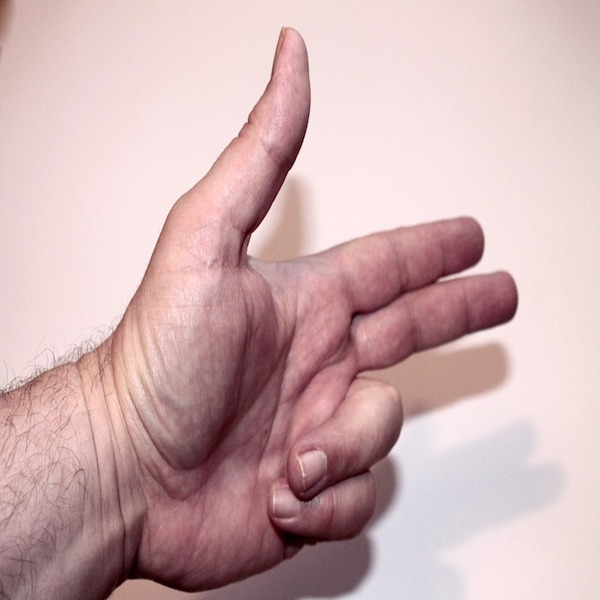
\includegraphics[width=40mm]{tfm-img1}}
\subfigure[Señal con luz]{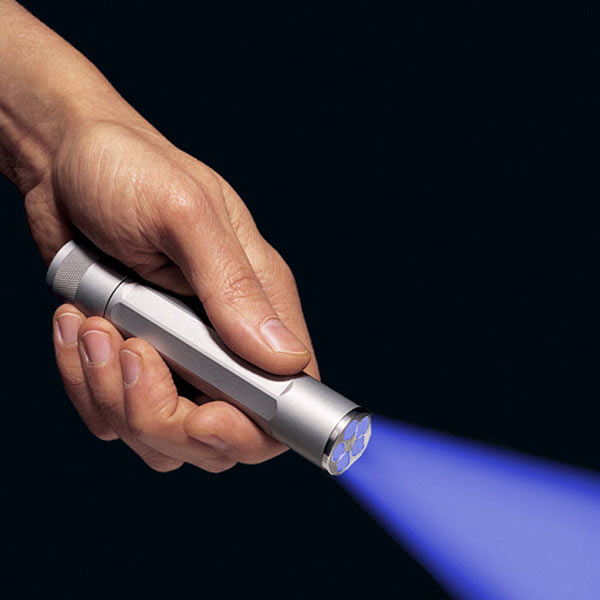
\includegraphics[width=40mm]{tfm-img2}}
\subfigure[Código escrito]{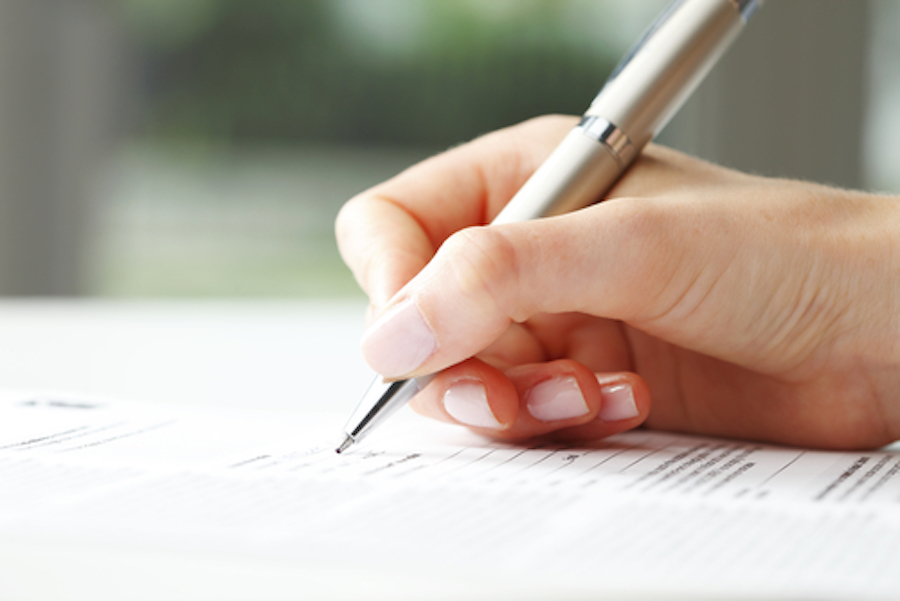
\includegraphics[width=80mm]{tfm-img3}}
\caption{Primeros sistemas de reconocimiento.} \label{fig:señales}
\end{figure}

Todos estos problemas fueron solventados con la aparición de la tecnología magnética. El que la información estuviese contenida en una banda magnética organizada en diferentes pistas hacía que no se pudiesen dar los casos sucedidos con los sistemas de reconocimientos tradicionales. En este ámbito, el uso de la tarjeta magnética era el medio utilizado en los sistemas de reconocimiento. Una tarjeta que poseía una banda magnética donde se almacenaba un código y que era leído a través de un lector con el que se podía extraer dicha información e identificar rápidamente a la persona que la portaba. Durante muchos años los sistemas de reconocimiento utilizaron este dispositivo como medio donde la información de identificación iba contenida. \\

\begin{figure}[htbp]
\centering
\subfigure[Tarjeta con banda magnética]{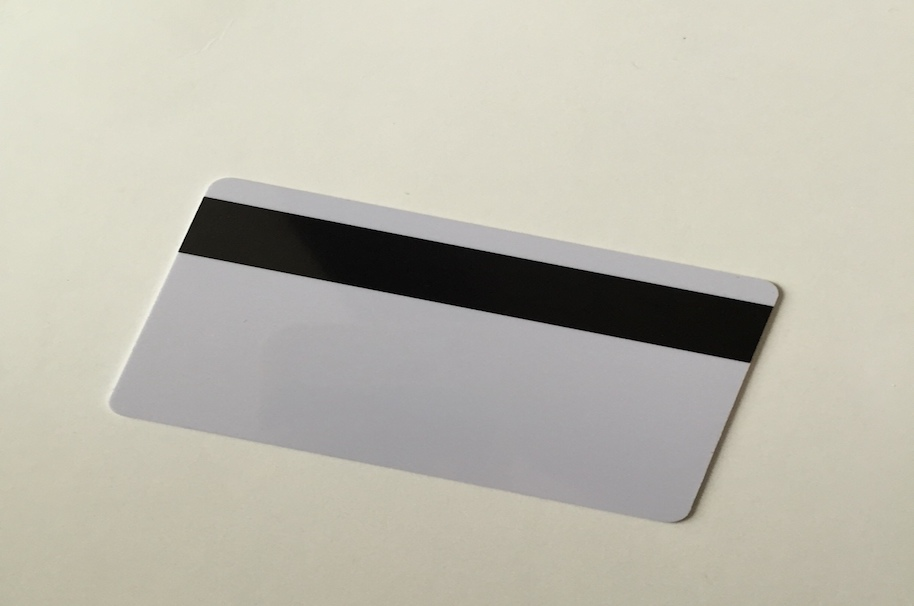
\includegraphics[width=50mm]{tfm-img4}}
\subfigure[Lector de tarjetas por banda magnética]{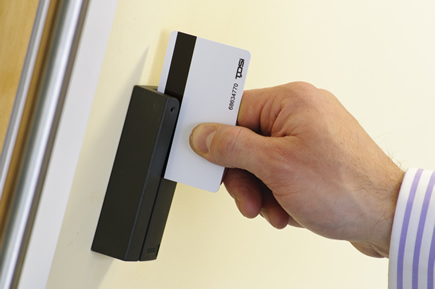
\includegraphics[width=50mm]{tfm-img5}}
\caption{La tecnología magnética en los sistemas de reconocimiento.} \label{fig:señales}
\end{figure}


El gran avance que experimentó la informática y la electrónica con el paso de los años hizo que los sistemas de reconocimiento a través de bandas magnéticas comenzasen a sufrir problemas de seguridad a raiz de la alta posibilidad que existía para suplantarlos. A este problema se unía el desgaste físico que se originaba en las bandas magnéticas a casua de su frecuente uso. Esto podía producir daño en la información almacenada en dichas bandas produciendo errores en la identificación. Fue en este punto cuando la tecnología digital apareció para dar solución a todos los inconvenientes que el uso de la tecnología magnética presentaba. La implantación de los chips digitales en los medios empleados por los sistemas de reconocimiento consiguieron dotar de una mayor seguridad y consistencia a estos sistemas, a la vez que hacía mas rápido todo el proceso de indentificación. Dispositivos como las tarjetas con banda magnética comenzaron incorporar este tipo de tecnología, al igual que los lectores tuvieron que actualizarse para extraer esa información. En este mismo entorno la tecnología digital progresó hasta la conexión entre dispositivos de manera inhalámbrica, es decir, los mismos dispositivos como las tarjetas se comunicaban con los lectores sin contacto físico, solo situándose a corto alcance. \\

\begin{figure}[htbp]
\centering
\subfigure[Tarjeta chip digital]{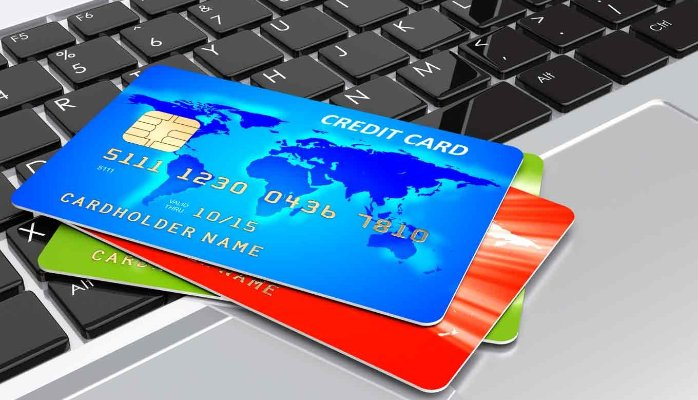
\includegraphics[width=44mm]{tfm-img6}}
\subfigure[Lector de tarjetas por chip digital]{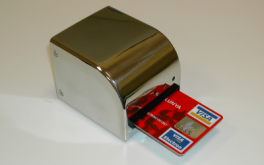
\includegraphics[width=40.1mm]{tfm-img7}}
\subfigure[Lector de tarjetas por chip digital wireless]{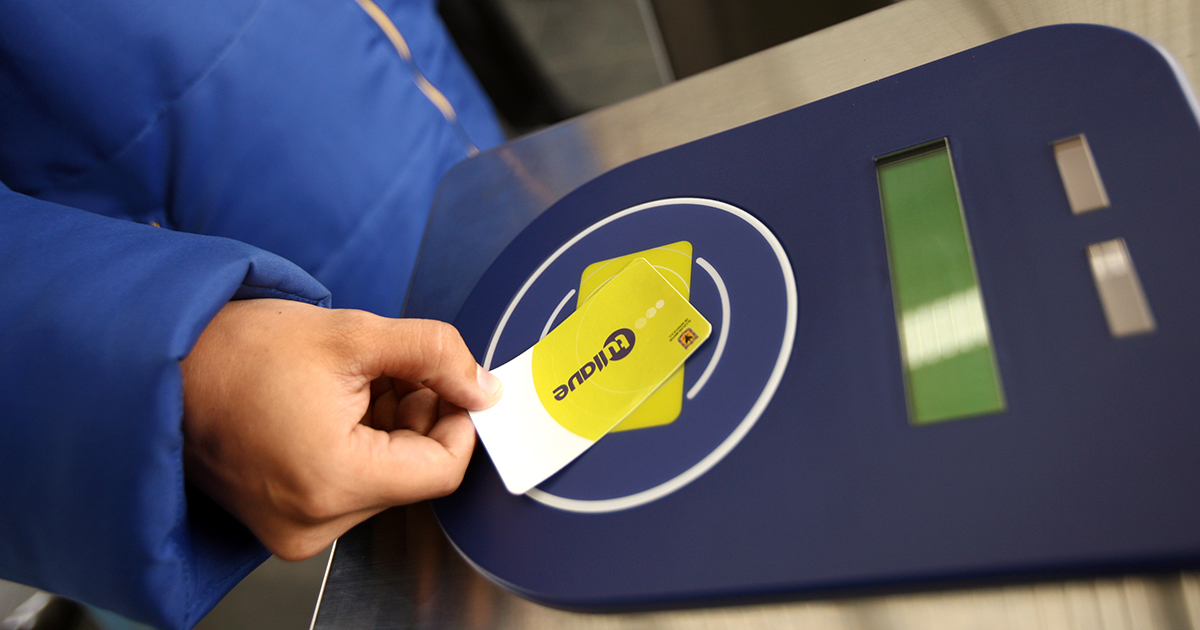
\includegraphics[width=80mm]{tfm-img8}}
\caption{La tecnología digital en los sistemas de reconocimiento.} \label{fig:señales}
\end{figure}

Nuevamente, la seguridad volvía a poner en duda los dispositivos empleados para contener la información de identificación de una persona. Los sistemas de reconocimiento basados en este tipo de dispositivos quedaban de esta manera expuestos a vulnerabilidades que podían desembocar en suplantaciones de indentidad. Todo esto era debido al gran avance tecnológico que se estaba produciendo, lo que hacía que sistemas que eran muy seguros en el momento de aparición de esa tecnología, con el paso del tiempo se conviertesen en obsoletos y débiles. Esto suponía que una nueva innovación en este sentido tendría una fuerte acogida al comienzo pero un nuevo declive con el paso del tiempo debido a los problemas de seguridad que se presentarían. \\

Este motivo hizo pensar en las características anatómicas que posee el ser humano como posible solución final a todos esos problemas. Esta propuesta cubría todas las condiciones que las anteriores no alcanzaban ya que presentaba propiedades de invariabilidad en el tiempo; lo que permitía que la persona mantuviera sus mismas características a lo largo de su vida, la imposibilidad de modificarlo o suplantarlo ya que son innatos a la persona que los tiene, etc. De todo esto surgió la idea de utilizar zonas del cuerpo humano como fuentes de información para los sistemas de reconocimiento a través de los patrones que estas describen. Así, partes de la fisiología de la persona como la huella dactilar, la retina, el iris, la palma de la mano e incluso la manera de andar constituían un gran almacen de datos que posibilitaría la identificación en los sistemas de reconocimiento. Con este nuevo medio de depósito de los datos, la seguridad, fiablidad y consistencia de la información aumentaba en los sistemas de información, quedando entonces del lado de ellos los errores que se produjeran por una mala identificación.  \\

El empleo de patrones de las características anatómicas del ser humano son la base de los actuales sistemas de reconocimiento. Estos se centran actualmente en mejorar los algoritmos empleados en el reconocimiento intentando conseguir una buena práctica y manejo de la información.   \\


\subsection{Reconocimiento de patrones}

El reconocimiento de patrones es la ciencia que se encarga de la descripción y clasificación (reconocimiento) de objetos, personas, señales, representaciones, etc. Esta ciencia trabaja en base un conjunto previamente establecido de todos los posibles objetos (patrones) individuales a reconocer. El ámbito de las aplicaciones basadas en el reconocimiento de patrones es muy amplio, siendo sin embargo las análogas al ser humano las que copan la mayor relevancia. El reconocimiento de patrones se da tanto en sistemas bióligicos como en sistemas dotados de inteligencia. Un claro ejemplo biológico lo vemos cuando en nuestro organismo los anticuerpos atacan a instrusos externos a los cuales reconoce a través del uso de patrones, en esta misma tesitura también se da el reconocimiento de patrones cuando nuestros oídos captan el habla y el sonido siendo capaz de interpretarlo. Del mismo modo, en situaciones que suceden en la naturaleza como cuando se produce la captura de las presas por parte de los animales se da el reconocimiento de patrones para conocer y diferenciar los tipos de presas. Este tipo de ejemplo llevado a los sistemas artificiales los podemos ver en los lectores de caracteres óptico (OCR) que son capaces de comprender el texto escrito y de como incluso las máquinas son capaces de enfrentarse a obstaculos y reconocer el diseño y características de estos. Cuando los patrones son de una naturaleza visual, el reconocimiento de patrones puede considerarse como un complemento en las técnicas de visión por computador proporcionando las capacidades de interpretación y clasificación \cite{Reference8}. \\

El reconocimiento de patrones esta ligado estrechamente con las redes neuronales. El nuevo interés a principios de los años 80 en las redes neuronales y el conexionismo como una alternativa al reconocimiento de patrones estadísticos y la inteligencia artificial (IA) puede atribuirse a dos factores. El primero es la realización que una función de aproximación de suficiente complejidad puede aproximarse a cualquier función objetivo con una precisión arbitraria. El segundo factor indica la capacidad para entrenar redes multicapas y no lineales usando backpropagation \cite{Reference8}. \\

Como se puede observar, el reconocimiento de patrones es la base teórica más importante de la biometría, de cómo esta busca la identidad de una persona en la forma de su mirada (la cara, la retina o el iris) o de algunas de sus zonas (las huellas dactilares o la geometría de la mano). En esencia, un sistema biométrico es un sistema de reconocimiento de patrones, razón por la cual el estudio de las bases matemáticas sobre las cuales se sustenta esta ciencia se vuelve de vital importancia para los fabricantes de tecnología biométrica. \\


\subsection{Componentes de los sistemas de reconocimiento de patrones}

El esquema de un sistema basado en el reconocimiento de patrones consta de varias etapas relacionadas entre sí (los resultados de una etapa pueden modificar los parámetros de etapas anteriores). La figura 2.4 muestra un esquema general de un sistema de reconocimiento de patrones en el cual el sensor tiene como propósito proporcionar una representación factible de los elementos del universo a ser clasificados en lo que se conoce como la etapa de adquisición de datos. Es conveniente realizar una etapa de preprocesamiento sobre cada uno de ellos en lugar de ser dados como entrada del sistema tal y como fueron obtenidos durante dicha etapa. La principal ventaja de realizar un preprocesamieno sobre los datos es que puede reducir la dimensionalidad de los mismos, lo cual mejora substancialmente la ejecución del sistema, sobre todo cuando se utiliza una metodología como la de redes neuronales. La extracción de características es la etapa que se encarga, a partir del patrón de representación de los datos, de extraer la información discriminatoria eliminando la información redundante e irrelevante. Es uno de los principales problemas que se dan en el reconocimiento de patrones, el encontrar una manera óptima de representar la información original que describe a cada uno de los patrones. Este proceso trata de reducir la cantidad de datos (reducción de dimensionalidad) que representa cada uno de los patrones, obteniendo de esta forma un vector de características que represente de la mejor manera posible al patrón original. El clasificador es la etapa de toma de decisiones en el sistema. Su rol es asignar los patrones de clase desconocida a la categoría apropiada. \\

En el caso de reconocimiento de patrones en imágenes la primera de las etapas, la adquisición de datos, generalmente es llevada a cabo mediante un dispositivo de captura de imagen, que se encarga de transformar la información obtenida del mundo real en un vector numérico que contiene los valores muestreados y cuantificados y que posteriormente es preprocesado. La etapa de selección y extracción de características es de suma importancia en un sistema de reconocimiento de patrones. Requiere un profundo análisis de los patrones para determinar que medidas son las cruciales en la identificación de las diferentes categorías. Durante esta etapa se aborda la recolección de información relevante proveniente de los dispositivos sensores para el proceso de clasificación. En el reconocimiento de patrones en imágenes se intenta extraer la información importante de las mismas en función del tipo de imagen, obviando siempre la que pueda ser intrascendente como el ruido. El objetivo final de un sistema de reconocimiento de patrones es la asignación automática de una categoría (o clase) a cada uno de los patrones de entrada \cite{Reference8}. \\

\begin{figure}[htbp]
\centering
\subfigure{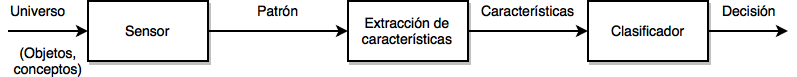
\includegraphics[width=140mm]{tfm-img9}}
\caption{Esquema general de un sistema de reconocimiento de patrones.} \label{fig:señales}
\end{figure}

El objetivo de estas etapas es ajustar el sistema para que sea capaz de clasificar señales u objetos de entrada en una de las clases predefinidas. Para ello deberá analizar un cierto número de características y para poder clasificar satisfactoriamente información de entrada es necesario un proceso de aprendizaje en el cual el sistema crea un modelo de cada una de las clases a partir de una secuencia de entrenamiento o conjunto de vectores de características de cada una de las clases. Generalmente se acepta que la secuencia de muestras de entrenamiento debe contener para cada una de las clases un mínimo de elementos igual a diez veces la dimensión de los vectores de características. El sistema de reconocimiento de patrones debe tener en cuenta las fuentes de variabilidad como son el ruido, rotaciones, cambio de escala y deformaciones, lo cual se logra incluyendo en la secuencia de entrenamiento patrones que hayan experimentado estas modificaciones. Este tipo de comportamiento se da en la etapa de clasificación, cuyo proceso de construcción suele denominarse como aprendizaje o entrenamiento, pudiendo ser este supervisado, en donde se realiza a partir de un conjunto de patrones del que no se conoce su clase; o no supervisado , los cuales requieren de la disposición de un conjunto de patrones denominado conjunto de entrenamiento, de los cuales se conoce su clase \cite{Reference8}.\\


\section{Biometría}

El concepto de biometría proviene de las palabras bio (vida) y metría (medida), refiriéndose por tanto a todo equipo biométrico que mide e identifica alguna característica propia de la persona. Se puede definir como una tecnología de seguridad basada en el reconocimiento de una característica física e intransferible de las personas, como por ejemplo la huella digital. Todos los seres humanos contienen características morfológicas únicas que los diferencian. La forma de la cara, la geometría de partes de nuestro cuerpo como las manos, nuestros ojos y tal vez la más conocida, la huella digital, son algunos rasgos que nos diferencian del resto de seres humanos.\\

La medición biométrica se ha venido estudiando desde hace mucho tiempo y es considerada en la actualidad como el método ideal y más fiable para la identificación humana. A través de la biometría se pueden medir y extraer las características anatómicas de una persona para obtener información y generar su patrón para poder emplearlo en su indentificación. \\


\subsection{Sistemas biométricos}

El gran avance que se ha producido en el desarrollo de las tecnologías de la información y la comunicación ha echo que sistemas tradicionales de reconocimiento como lectores de tarjetas, número secreto, etc. hayan adoptado esta evolución para dar paso a los sistemas biométricos. La autenticación mediante verificación biométrica está convirtiéndose en algo cada vez más habitual en los sistemas de seguridad, tanto privados como públicos, en la electrónica de consumo y en las aplicaciones de punto de venta (POS). Además de la seguridad, otro de los factores que está impulsando la verificación biométrica es la comodidad. \\

Un sistema biométrico se basa en las características que aporta la anatomía del ser humano, fundamentando sus desiciones de reconocimiento mediante los patrones que estas forman. Estos patrones son características morfológicas únicas y de comportamiento que todos los seres humanos tenemos y que nos diferencian de los demás. Propiedades como la forma de la cara, la geometría de partes de nuestro cuerpo como las manos nuestros ojos y la huella digital, son algunos rasgos que nos diferencian del resto de seres humanos.\\

Los sistemas biométricos pueden ser clasificados de diferentes maneras. Dependiendo del tipo de característica que se utilice para llevar a cabo de la identificación biométrica los podemos clasificar en dos grandes tipos; la biometría estática y la biometría dinámica. \\

La biometría estática engloba todas las características físicas que posee la persona como la huella dactilar, el iris del ojo, la palma de la mano, la cara, la oreja, etc. mientras que la biometría dinámica se basa en las características de comportamiento como la escritura, la firma, etc. 
Otra clasificación de los sistemas biométricos la podemos basar en el tipo de tecnología biométrica sobre la que se basan, donde podemos encontrar el reconocimiento de huella dactilar, reconocimiento de iris, reconocimiento de la geometría de la mano, reconocimiento de firma escrita y reconocimiento de voz.\\

Por la cuota de mercado que tienen estas tecnologías biométricas podemos clasificarlas según la información proporcionada por el International Biometric Group en el estudio realizado en enero de 2016 donde muestra la proporción del consumo de los diferentes tipos de sistemas biométricos.\\

\begin{figure}[htbp]
\centering
\subfigure{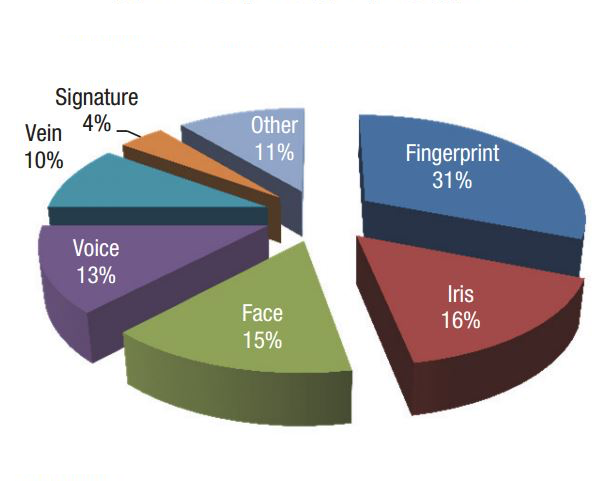
\includegraphics[width=80mm]{tfm-img10}}
\caption{Cuota de mercado de las modalidades de sistemas biométricos.} \label{fig:señales}
\end{figure}

En la figura anterior podemos ver como el reconocimiento por huella dactilar es el sistema biométrico más utilizado en el mercado por las aplicaciones de seguridad, teniendo el resto de tecnologías biométricas un alcance similar en cuanto al consumo. Esto no hace más que representar el desafío que supone el analizar e investigar un sistema biométrico que no esta tan asentado en el mercado como es el basado en el iris, y que puede conllevar a obtener nuevos hallazgos y soluciones que mejoren las capacidades de lo ya existente.


\subsection{Anatomía del iris}

El ojo es el órgano de la visión. Los ojos pueden distinguir variaciones muy pequeñas de forma, color, luminosidad y distancia. En realidad, el órgano que efectúa el proceso de la visión es el cerebro; la función del ojo es traducir las vibraciones electromagnéticas de la luz en un determinado tipo de impulsos nerviosos que se transmiten al cerebro. \\

El ojo en su conjunto, llamado globo ocular, tiene un diámetro aproximado de 2,5cm con un marcado abombamiento sobre su superficie delantera. Entre la pared del globo ocular y el hueso orbitario existe un tejido conjuntivo que une ambas estructuras. A dicha zona de unión se le conoce como cápsula de Tenon. \\

El ojo se compone de una serie de estructuras entre la que destacamos el iris, una membrana coloreada y de forma circular. Su coloración representa lo que conocemos habitualmente como “color de los ojos” y su apertura central es la pupila. Esta membrana presenta un músculo de disposición circular que permite modificar el tamaño de la pupila.\\

El iris forma parte de la capa media o úvea. Es un disco pigmentado que se encuentra a continuación del cuerpo ciliar, suspendido entre la córnea y el cristalino. Posee un orificio central conocido como pupila por donde pasan los rayos lumínicos tras haber atravesado la córnea y el humor acuoso. A través de la pupila los rayos llegan a la lente del cristalino, seguidamente al cuerpo vítreo y finalmente a las células receptoras de la retina para la formación de la imagen. El tamaño de la pupila depende de dos músculos que rodean sus bordes y controlan la cantidad de luz que entra en el ojo. Las fibras musculares del iris se agrupan formando dos músculos obiculares: el Esfínter del iris que produce la Miosis, y el dilatador de la pupila que produce la Midriasis. Si los músculos orbiculares del iris se contraen, la pupila se encoge y entra menos luz en el ojo (Miosis). Si los músculos orbiculares se relajan, la pupila vuelve a dilatarse, dejando pasar más luz a la retina (Midriasis).  La contracción pupilar se debe  a la acción de los esfínteres del iris y su objetivo es dar una imagen nítida, evitando para ello el paso de rayos por la periferia de la lente. El componente principal del iris es un tejido conjuntivo rico en células pigmentadas llamadas melanóforos.\\

Se encuentra situado entre la cámara anterior y posterior de un líquido gelatinoso llamado humor acuoso. La cámara anterior esta delimitada por la cara posterior de la córnea y la cara anterior del iris, mientras que la cámara posterior lo está por la cara posterior del iris y la cara anterior del cristalino. Posterior al cristalino se encuentra el humor vítreo que da volumen al globo ocular. \\

\begin{figure}[htbp]
\centering
\subfigure{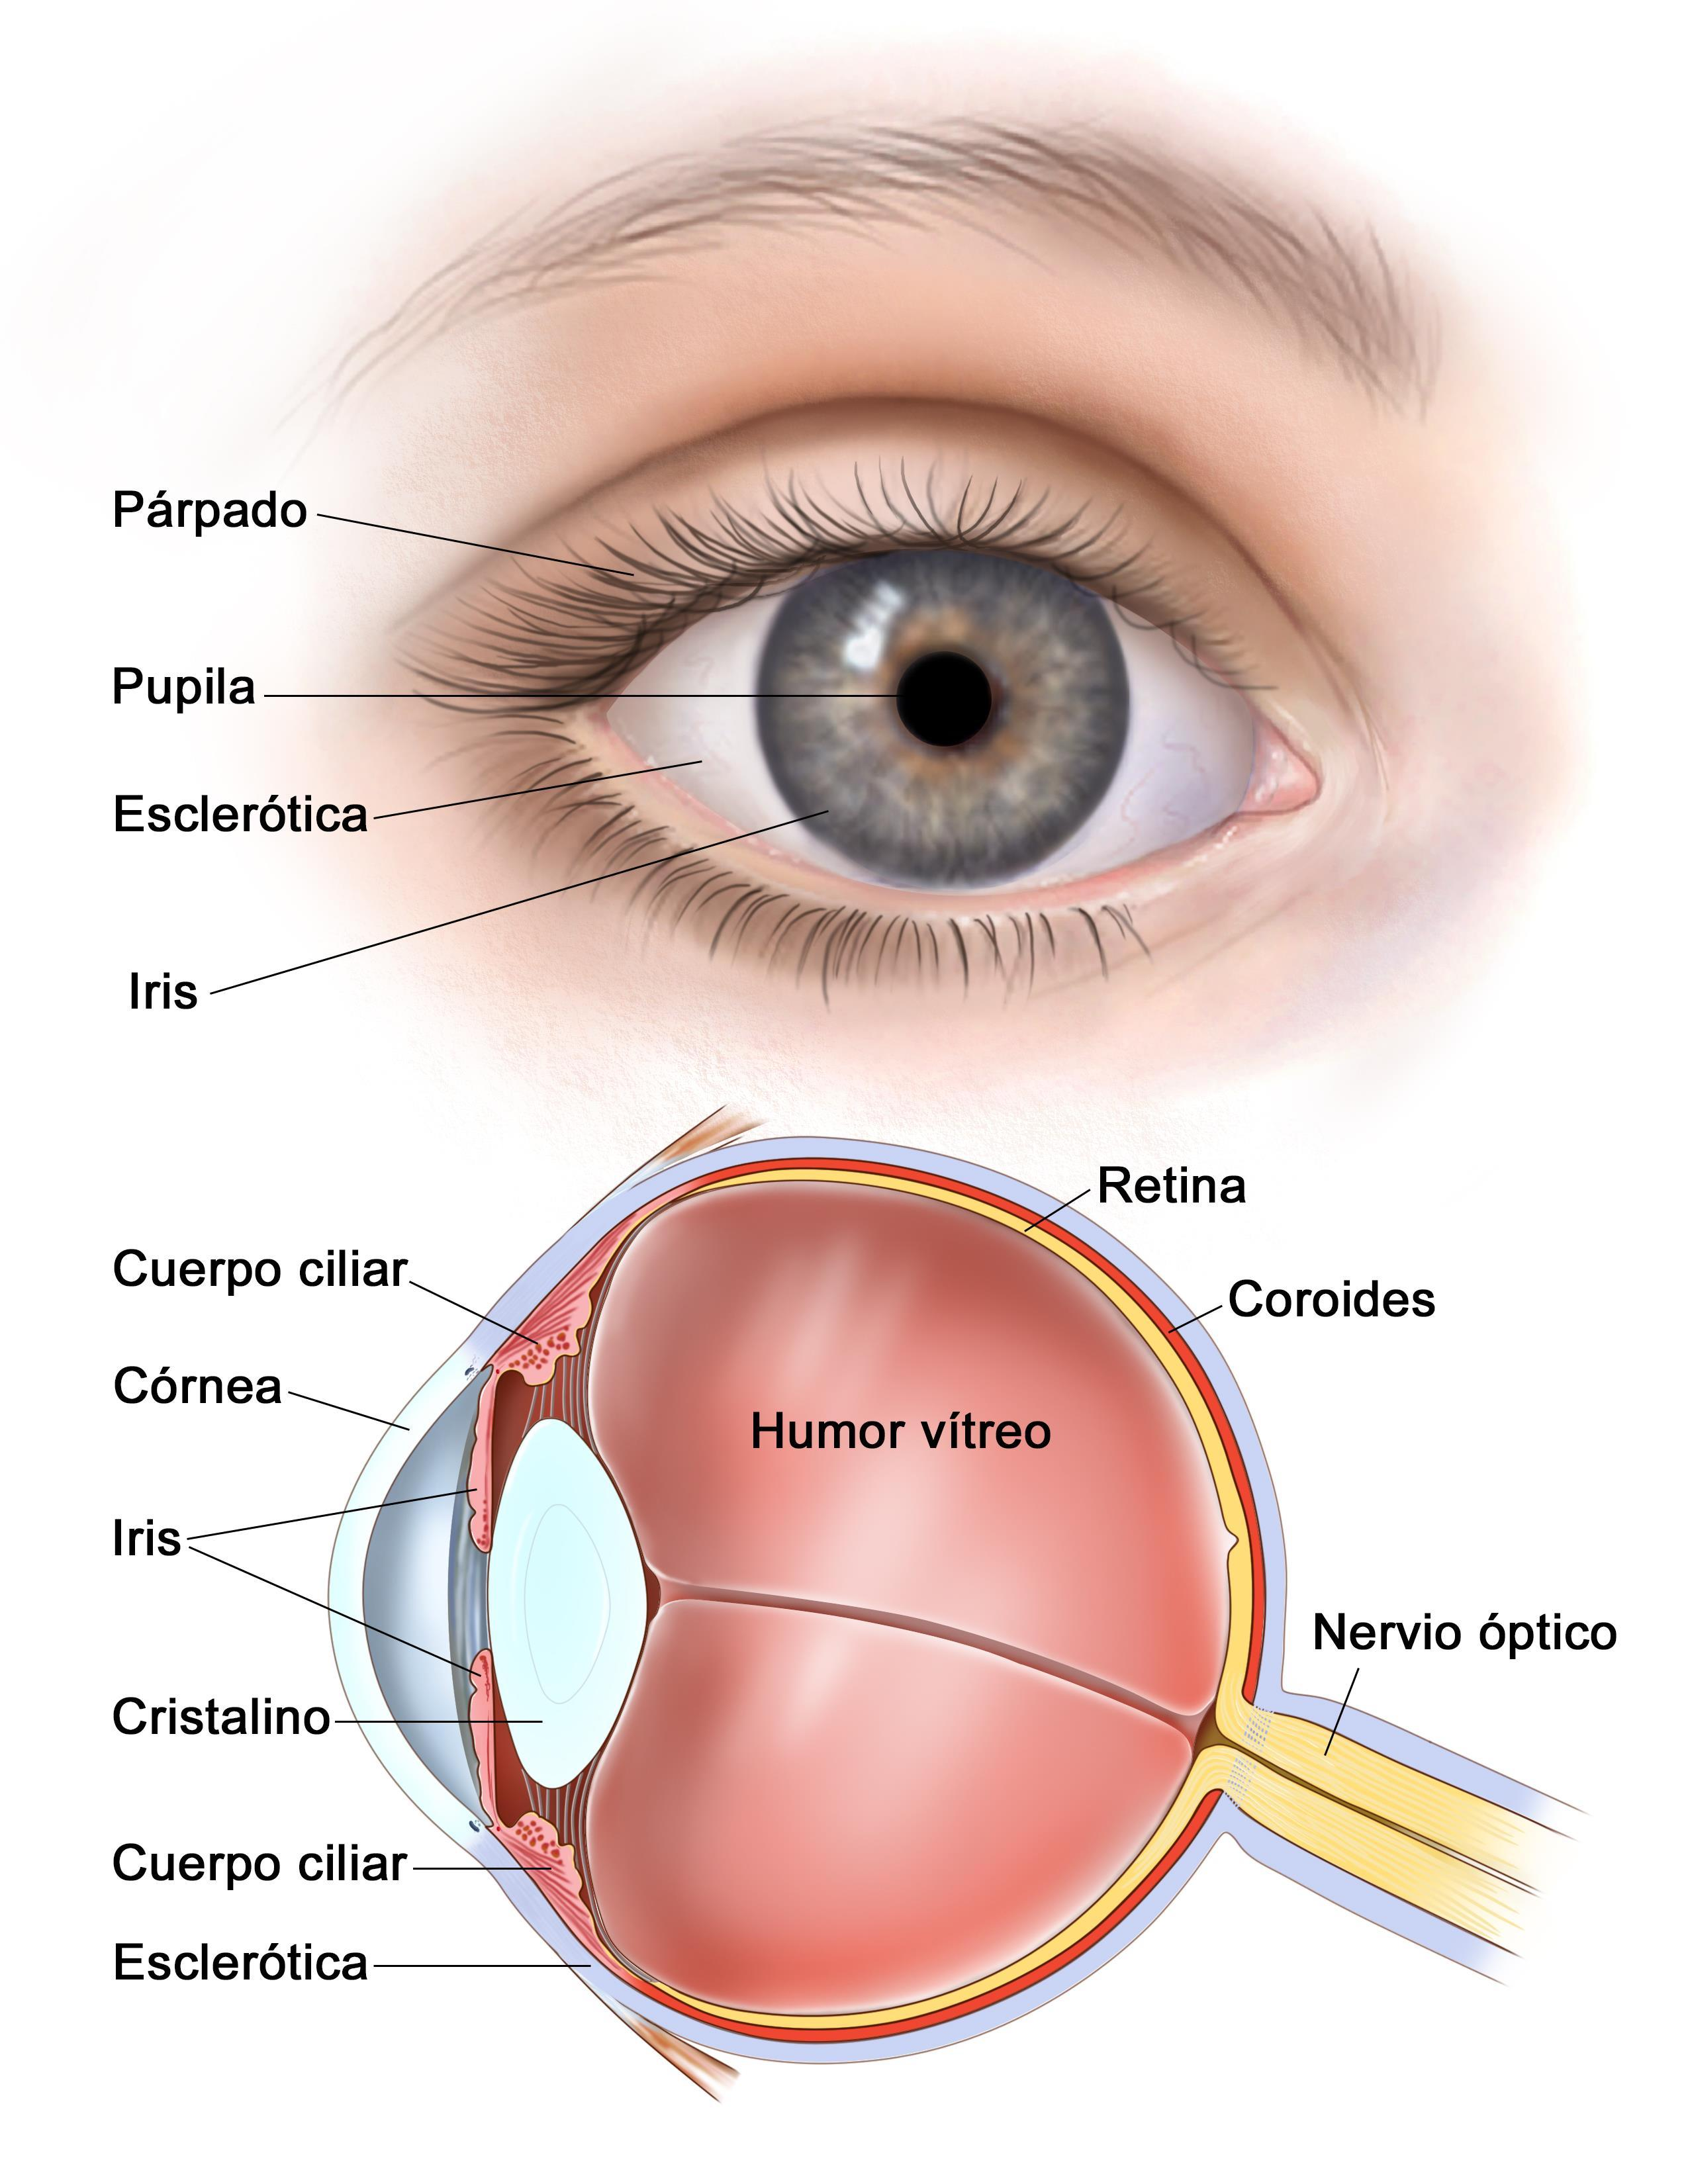
\includegraphics[width=80mm]{tfm-img11}}
\caption{Anatomía del iris.} \label{fig:señales}
\end{figure}

El iris es una zona delicada del ojo y que está expuesta a sufrir posibles daños y enfermedades. Los traumatismos son la causa mas frecuente de cataratas unilaterales en individuos jóvenes. Una herida contusa por la cual una contusión puede dar lugar a una “impronta” del pigmento del iris sobre la cápsula anterior del cristalino, así como opacidades corticales con forma de flor. La mayor temperatura del iris respecto a la de la córnea puede formar corrientes en termoconvección en el humor acuoso que ascienden y descienden cerca del iris y endotelio respectivamente. Son típicos en la mitad inferior de la córnea formando un triángulo con base inferior. El crecimiento o protuberancia en la superficie anterior del iris, que no son sino cúmulos inflamatorios en el parénquima iridiano, puede dar lugar a la enfermedad denominada Nódulos de Bussaca. \\

El color del iris está determinado por el número y distribución de unas células que contienen el pigmento Melanina y se llaman Melanocitos. Si la melanina se encuentra solamente en la zona de epitelio pigmentario de la superficie posterior del iris, el ojo es azulado. En cambio si esta se distribuye por todo el espesor del iris, el ojo es de color marrón. \\


%----------------------------------------------------------------------------------------


\section{Reconocimiento de iris}

A pesar de no ser el tipo de reconocimiento que mayor uso tiene en el mercado, este tipo de reconocimiento presenta una gran popularidad debido a las propiedades que posee como son principalmente los muchos grados de libertad con los que es dotada su textura, y el permanecer invariable en el tiempo a pesar del envejecimiento natural de la persona. Todo esto convierte al iris en una de las mas importantes características de la fisiología humana que da lugar a un sistema de reconocimiento biométrico robusto, fiable u seguro. \\

El proceso de reconocimiento de iris se compone de cuatro etapas principales: la adquisición de imagen, el pre-procesamiento, la  extracción de características y la comparación de las mismas. Estas cuatro fases constituyen una arquitectura de flujo de trabajo pipeline, donde el resultado de la salida de un etapa es la entrada en la inmediatamente posterior.\\

\begin{figure}[htbp]
\centering
\subfigure{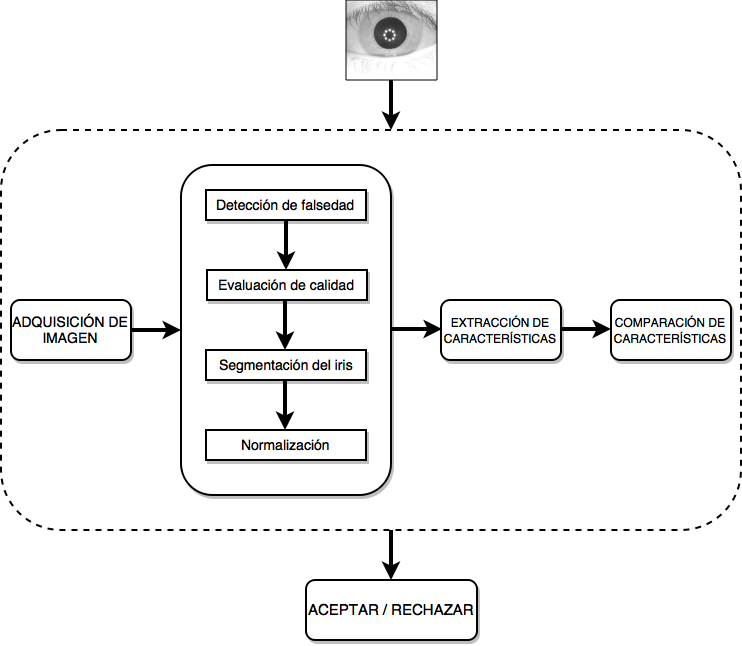
\includegraphics[width=130mm]{tfm-img12}}
\caption{Diagrama de flujo de un sistema de reconocimiento de iris.} \label{fig:señales}
\end{figure}


\subsection{Etapas del reconocimiento de iris}

Un sistema de reconocimiento basado en el iris se compone de cuatro etapas: adquisición de imagen, pre-procesamiento, extracción de características y comparación de características. En la figura 2.7 podemos ver el digrama del flujo de ejecución de un sistema de reconocimiento de iris convencional, los cuales comienzan con la adquisición de la imagen del iris y terminan aceptando o rechazando la identidad reclamada. \\

La primera etapa de adquisición de imagen es la encargada de capturar una secuencia de imágenes de iris. Estas capturas se realizan con cámaras especiales que suelen operar en el espectro visible (380-750 mm) o en el espectro infrarrojo (700-900 mm). En este ámbito, los sistemas de adquisición en el espectro infrarrojo son los más utilizados debido a las ventajas que proporciona. Dicho proceso de adquisición consiste en 2 operaciones: muestreo y cuantización. El muestreo está relacionado con la creación de la imagen digital, que tiene una resolución espacial predefinida con un número de pixeles por pulgada en función de la escena donde se realice. A través de la operación de cuantización, la señal de entrada es discretizada para obtener los posibles valores de intensidades de los pixeles que conforman la imagen. \\

La etapa de pre-procesamiento es la segunda y como se ha podido ver en la figura 2.7 se compone a su vez de 4 sub-etapas: detección de falsedad, evaluación de calidad de la imagen, segmentación del iris y normalizaciónd de la región del iris. La detección de falsedad es empleada para diferenciar entre un reclamo de identidad real y un falso reclamo con una imagen impresa de un iris, una grabación de secuencia de vídeo de un iris, ojos artificiales, lentes de contacto impresos con patrones de iris por ejemplo. Para detectar esa falsedad de identidad se emplean técnicas de medición de indicadores de espécimen vivo. La sub-etapa de evaluación de calidad dentro de la etapa del pre-procesamiento involucra varios factores de calidad como son: emborronado por desenfoque, emborronado por movimiento, dilatación de la pupila, área útil del iris, reflexiones especulares, variaciones de iluminación, oclusión por pestañas y párpados. Una pronta detección y corrección de estos factores de calidad ayudará a que el proceso de reconocimiento del iris sea mas robusto, aunque existen muchos sistemas de reconocimento de iris que imponen una serie de restricciones en la etapa de adquisición de la imagen del iris teniendo como objetivo el reducir dichos factores de calidad. \\

La segmentación del iris se compone también de una serie de pasos: encontrar un iris en la imagen, demarcar sus bordes interno y externo entre la pupila y la esclerótica respectivamente, detección de los bordes de los párpados superior e inferior si estos ocluyen el iris, y detectar y excluir cualquier objeto superpuesto de pestañas o reflexiones de la córnea o gafas. Existen diferentes métodos propuestos de segmentación de iris como: método basado en el operador integro-diferencial, método basado en la transformada de Hough, método basado en el análisis de contornos activos, método basado en la teoría de juegos, etc. Con el paso de la normalización de lo que se trata es de solucionar los problemas relacionados con las dimensiones de la imagen del iris. La dimensión de la imagen del iris puede variar de un individuo a otro o en el mismo individuo debido a la variación de la pupila, la variación de la distancia entre el individuo y la cámara, el movimiento del ojo, la inclinación de la cabeza, etc. Con el proceso de normalización lo que se hace es transformar la región segmentada del iris en un sistema de coordenadas pseudo-polar de 2 dimensiones mediante un muestreo de los datos originales en un tamaño predefinido. Aunque en algunos modelos del desarrollo de extracción de características no se realiza este proceso para ahorrar en coste computacional, el modelo "rubber sheet" es el método mas usado para la normalización \cite{Reference9}. \\

En la siguiente etapa se extraen las características mas significativas y relevantes de la textura de la imagen del iris. Este proceso se ha desarrollado utilizando diversos algoritmos de codificación entre los que se pueden destacar: banco de filtros espaciales, transformada de Gabor wavelets en 2 dimensiones, transformada discreta de los cosenos, transformada discreta de Fourier en 2 dimensiones, características ordinales, descriptores SIFT alrededor de un punto de interés, etc. El éxito de las estapas de segmentación y extracción de características se encuentra estrechamente ligado a los factores de calidad de la imagen del iris, por lo que como se ha mencionado anteriormente, una buena etapa de pre-procesamiento puede evitar que se dé el caso en el que usuarios auténticos  con imágenes capturadas con mala calidad puedan ser injustamente rechazados ya que difieren de sus plantillas biométricas registradas. \\

Por último, en la etapa de comparación de característica se confirma si la imagen de la textura del iris de un individuo dado se corresponde a algunas de las identidades registradas por el sistema. Esta operación de similitud se desarrolla utilizando diferentes medidas de similitud propuestas en función de la magnitud de las características extraidas. Mediante estas medidas de magnitud se puede decidir si la identidad reclamada es aceptada o rechazada. Entre las medidias más utilizadas en la comparación de características de la textura del iris se pueden destacar: distancia euclidiana, distancia de Hamming o la función BLPOC \cite{Reference9}.\\


\section{Reconocimiento de iris en condiciones no ideales}

La mayor parte de los trabajos realizados sobre el reconocimiento del iris alcanzan muy buenos resultados que se convierten en casi inalcanzables en ambientes deseados. Como se ha mencionado anteriormente, en la actualidad son muchas las investigaciones que se centran en el desarrollo de métodos robustos capaces de realizar un reconocimiento del iris en ambientes no deseados o condiciones no ideales. La tendencia de esta modalidad de reconocimiento biométrico viene promovida por la necesidad de algunas aplicaciones reales para obtener una mayor flexibilidad frente a situaciones como: seguimiento de personas, reconocimiento de personas en multitudes, control de acceso, etc, donde la aparición de factores de calidad como iluminación, escala, oclusión y/o perspectiva convierten el entorno del reconocimiento en no deseado, teniéndose este que realizar en condiciones no ideales. A pesar del gran avance de los desarrollos producido en este campo, existen actualmente grandes retos en cuanto al reconocimiento de iris en condiciones no ideales \cite{Reference9}.\\

El reconocimiento del iris en condiciones no ideales se caracteriza por manifestarse en situaciones donde el individuo se encuentra en constante movimiento o en escenarios con presencia de objetos y/u otros individuos, lo que provoca que se realicen capturas de imágenes del iris afectadas por factores de calidad. Se suelen dar una serie de factores de calidad comunes a las imagenes capturadas este tipo de situaciones como son la iluminación variable, el emborronado, la oclusión, la reflexión especular, el tamaño del área del iris y la perspectiva. \\
 
La existencia de estos factores de calidad en las imagenes del iris pueden producir que la medida de éxito de los sistemas de reconocimiento se vea afectada negativamente. Por este motivo suelen aperecer una serie decisiones que se pueden tomar para intentar mitigar este problema como son el descartar las imagenes que no superen un umbral de índice de calidad establecido, el aplicar técnicas para mejorar la calidad de las imágenes, el desarrollar técnicas mas robustas de reconocimiento de iris en imagenes de mala calidad y el obtener combinaciones de estas técnicas \cite{Reference9}.\\

\begin{figure}[htbp]
\centering
\subfigure{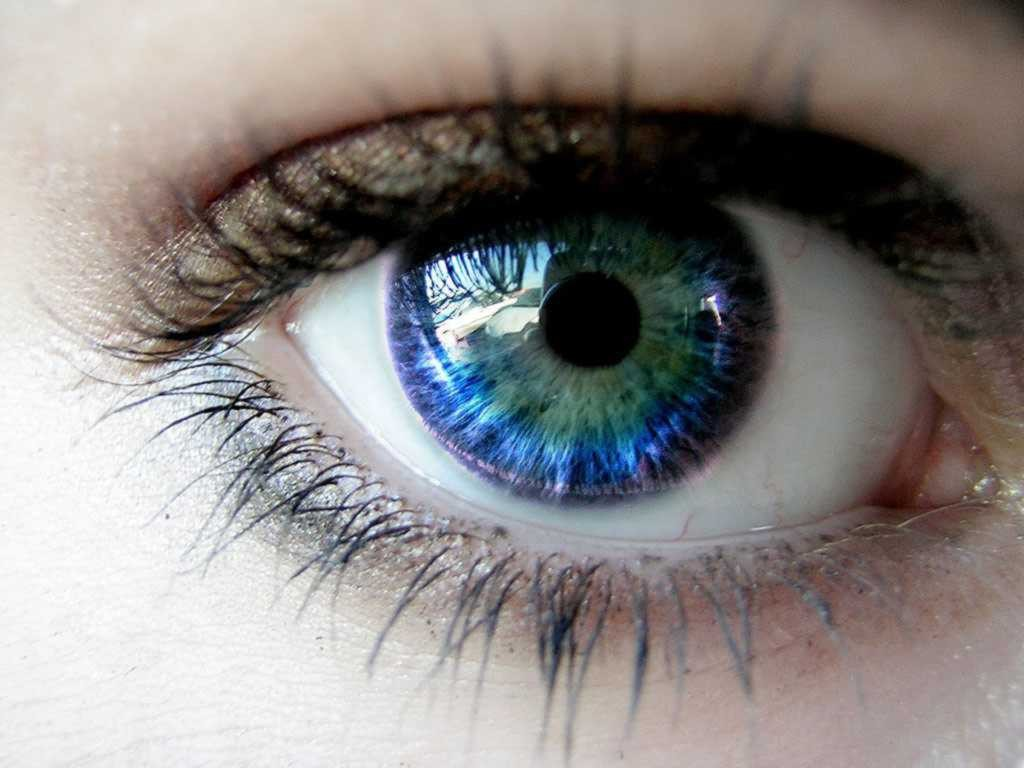
\includegraphics[width=44mm]{tfm-img13}}
\subfigure{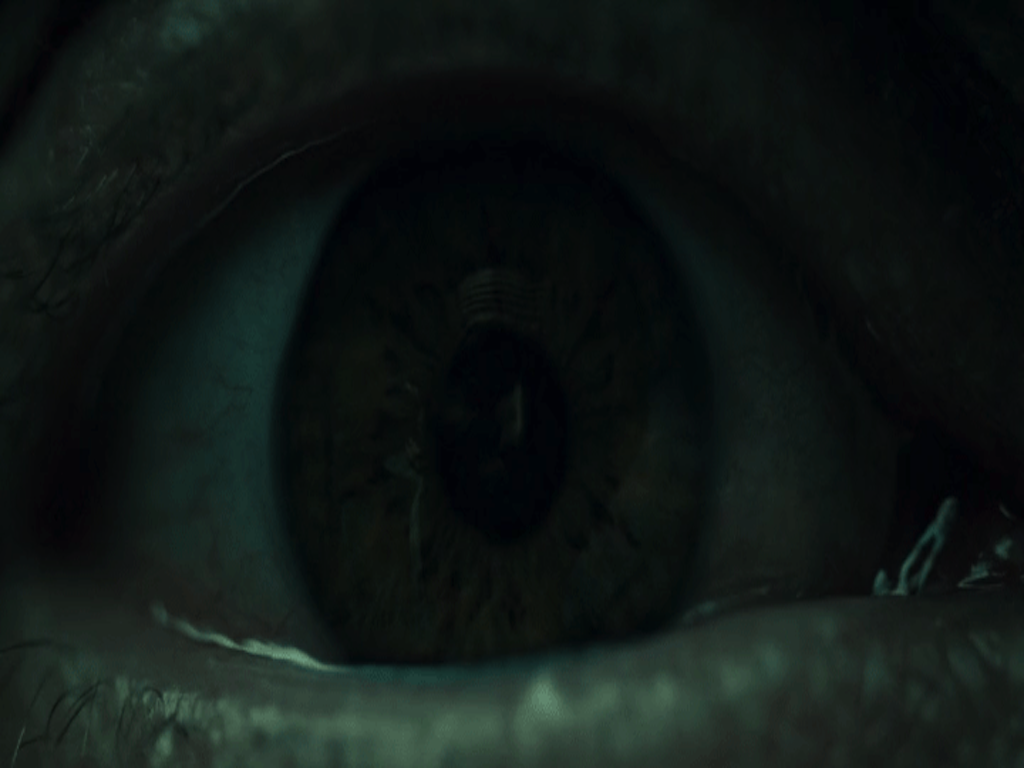
\includegraphics[width=44mm]{tfm-img14}}
\subfigure{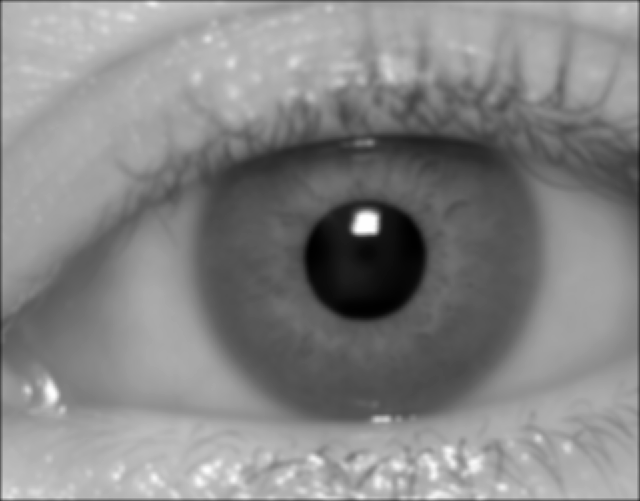
\includegraphics[width=60mm]{tfm-img15}}
\caption{Imágenes de iris afectadas por factores de calidad.} \label{fig:señales}
\end{figure}


\subsection{Factores de calidad}

En esta sección describiremos los factores de calidad más comunes que suelen aparecer en las imágenes de textura del iris cuando estas se realizan en movimiento o con la presencia de objetos y/o personas. \\

La iluminación variable es un problema que está estrechamente ligado a la localización de la fuente de luz con respecto al dispositivo de captura y el individuo que se quiere reconocer. Estas variaciones de iluminación están siempre relacionadas al movimiento de la persona con respecto a las fuentes de luz. Debido a esto, la intensidad y la dirección de las fuentes de iluminación pueden afectar la apariencia de imágenes del iris e indicir en las medidas de éxito de los sistemas de reconocimiento de iris. Algunos sistemas de reconocimiento emplean el uso de filtros ópticos para reducir el efecto de la luz variable, ya que estos bloquean con luz estroboscópica una gran porción de luz ambiental. La aplicación de técnicas de ecualización de histogramas y  de estandarización es otro método utilizado para disminuir el efecto contraproducente de la variabilidad luminosa. \\

Como hemos visto en la sección \textbf{Anatomía del iris}, este se representa como un anillo que tiene el borde inferior situado sobre la pupila y el borde exterior sobre la esclerótica, siendo su función principal la de controlar el tamaño de la pupila en función de la cantidad de luz que entra en el ojo a través de esta.  Esa cantidad de luz puede dar lugar a que se den dos fénomenos en la pupila; la "Miosis" debido a que la pupila se contrae por el exceso de cantidad de luz y la "Midriasis" que se dilata por el efecto contrario, es decir, poca cantidad de luz. La variabilidad de tamaño de la pupila hace el tamaño de la región del iris pueda variar. \\

En situaciones en las que se capture la imagen del iris con mucha cantidad de luz provocará que la pupila esté dilatada, dando lugar a que no se obtenga la información necesaria para realizar el proceso de reconocimiento. Esto es debido a que la dilatación de la pupila produce una deformación y pérdida de información relevante del patrón estructural del iris \cite{Reference9}.\\

El problema que produce el efecto de emborronado sobre las imágenes es causado principalmente por 2 motivos como son los movimientos significativos del individuo respecto al dispositivo de captura o del dispositivo de captura respecto al individuo en el momento de la adquisición de la imagen y que el punto focal del objeto a capturar esté fuera de la profundidad del campo del dispositivo de captura de la imagen. Para paliar este problema se han desarrollado soluciones basadas en enfoques de estabilización opto mecánica que va incorporada en el ensamblado de las lentes de las cámaras utilizando un software conectado con un control electrónico de imagen. Estas soluciones implican la incorporación de dispositivos costosos y voluminosos que no serían viables para ser utilizados en aplicaciones móviles. En este sentido, se han propuesto varios métodos que permiten entre otras cosas  determinar el nivel de afectación de emborronado  en las imágenes, así como medir el foco de una imagen por el análisis de la nitidez del límite entre el iris y la pupila. \\

Otro de los factores de calidad que se puede dar en las imágenes de captura de iris es el referente a la oclusión ocasionada por los párpados y pestañas, las cuales pueden ser parciales o totales. En este caso, en las oclusiones parciales se puede comprobar como la oclusión al iris se produce mayormente por el párpado y las pestañas superiores. Esta situación es muy común en los seres humanos, ya que con el paso de los años el párpado tiende a caerse y con ello a obstruir el ojo. Por otro lado, las oclusiones totales se deben en parte a algún tipo de enfermedad padecida por el individuo o alguna fuerte reacción a cambios en el ambiente. El efecto de oclusión provoca que se capturen imágenes que proporcionen poca o ninguna información de los patrones estructurales del iris, afectando con ello a la medida de éxito de los sistemas de reconocimiento de iris \cite{Reference9}.\\

Al igual que con los anteriores factores de calidad, son varias las soluciones desarrolladas para la detección de párpados y pestañas entre los que se encuentran el método de detección de párpados y pestañas basado en las transformada de Hough \cite{Reference10} o el método de detección de párpados basado en características de las frecuencias de las pestañas \cite{Reference11} entre otros. \\

La reflexión especular es un factor de calidad que viene asociado a los mecanismos de iluminación que traen incorporados los dispositivos de captura de imagen del iris para iluminar el ambiente en el que se encuentra el individuo que vaya a ser reconocido para poder capturar imágenes de iris con mayor calidad y grado de detalle posible. Este medio propicia que se produzcan reflexiones de luz sobre la córnea del ojo del individuo. Estas reflexiones especulares pueden ser definidas como manchas blancas que ocluyen y esconden información del iris y la pupila. Esta oclusión de información por parte las reflexiones especulares sobre el iris puede provocar que se altere el patrón estructural de este, llegando en ocasiones a no poder localizarlo. Esto puede ocasionar que un individuo sea rechazado por el sistema de reconocimiento aún estando registrado por dicho sistema \cite{Reference9}. \\

Existen varias soluciones para evitar que aparezcan reflexiones especulares en las imágenes del iris, siendo una de ellas la de controlar la iluminación ambiental con iluminación NIR. Aunque otros trabajos desarrollados proponen otro tipo de soluciones basados en un sistema con una fuente de luz menos invasiva diseñado para eliminar reflexiones especulares \cite{Reference12}. \\

El factor de la perspectica se encuentra relacionado con la desviación de la mirada del individuo a reconocer respecto a la vista frontal ideal desde el dispositivo de captura. Este factor tiene una enorme influencia sobre la medida de éxito de los sistemas de reconocimiento de iris, ya que las imágenes de iris con desviaciones respecto a la vista frontal ideal tienen la característica de que el iris capturado posee una forma elíptica. Esto hace que el patrón estructural del iris tienda a deformarse significativamente, lo que produce que la información capturada del mismo no coincida con el modelo estructural de un iris normal \cite{Reference9}. \\  

Existen varios trabajos desarrollados para procesar este tipo de imágenes como el propuesto por J. Zhu y J. Yang \cite{Reference13} basado en la estimación de la dirección de la mirada sobre el análisis de secuencias de vídeo, y también Dorairaj et al. en \cite{Reference14} estiman el ángulo de desviación de la mirada repecto a la vista frontal ideal optimizando una función objetivo basada en la distancia de Hamming \cite{Reference15}. \\

%---------------------------------------------------------------------------------------- 
% Chapter 3

\chapter{Tecnologías y herramientas en el reconocimiento de iris} % Main chapter title

\label{Capítulo 3} % For referencing the chapter elsewhere, use \ref{Chapter3} 

%----------------------------------------------------------------------------------------

% Define some commands to keep the formatting separated from the content 
%\newcommand{\keyword}[1]{\textbf{#1}}
%\newcommand{\tabhead}[1]{\textbf{#1}}
%\newcommand{\code}[1]{\texttt{#1}}
%\newcommand{\file}[1]{\texttt{\bfseries#1}}
%\newcommand{\option}[1]{\texttt{\itshape#1}}

%----------------------------------------------------------------------------------------

\section{Introducción}

Conocida ya la práctica general de los sistemas de reconocimiento de personas y de manera mas específica los basados a través del iris que se ejecutan en condiciones no ideales, en este capítulo vamos a estudiar las herramientas y tecnologías existentes en las que nos apoyaremos para desarrollar un nuevo método de extracción de características que sea integrado en un sistema de reconocimiento de este tipo con el objetivo de evaluar su rendimiento comparando sus resultados con los obtenidos usando diferentes métodos de extracción de características. \\

Como bien hemos podido ver en el capítulo anterior, un sistema de reconocimento biométrico se compone de cuatro elementos principales: la adquisición de imágenes, el pre-procesamiento, la extracción de características y la comparación de las mismas. Aunque el propósito de este Trabajo Fin de Master es el de diseñar e implementar un nuevo método de extracción de características, también será necesario desarrollar el resto de componentes que forman un sistema de reconocimiento biométrico para evaluar los resultados, haciendo uso para ello de las herramientas que se describen en este apartado.\\ 

Para la etapa de adquisición de imágenes haremos uso de la base de datos \textbf{CASIA V4} \footnote{Disponible en el sitio web de CASIA (http://biometrics.idealtest.org)}, la cual contiene un conjunto de imágenes tomadas a individuos de los ojos izquierdo y derecho afectadas por diferentes factores de calidad. Para el resto de las etapas se emplearán las diferentes librerías y frameworks que se mencionan a continuación. Mediante la librería \textbf{USITv1.0.3} \footnote{Disponible en el sitio web de USIT (http://www.wavelab.at/sources/USIT/)}, la cual se basa en \textbf{OpenCV} \footnote{Disponible en el sitio web de OpenCV (http://opencv.org)} y \textbf{Boost} \footnote{Disponible en el sitio web de Boost (http://www.boost.org)} se desarrollarán las etapas de pre-procesamiento y comparación de características. Del mismo modo, la etapa de extracción de caracterísitcas se basará en el framework de desarrollo \textbf{LIP-VIREO} \footnote{Disponible en el sitio web de LIP-VIREO (https://code.google.com/archive/p/lip-vireo/)}, ya que este nos proporciona una amplia variedad de diferentes métodos de extracción de características que serán los que se empleen para obtener los diferentes resultados que serán cotejados en la etapa de comparación. \\

El desarrollo del método de extracción de características sobre el que se basa esta memoria se apoyará en la librería \textbf{LIP-VIREO}. \\



%----------------------------------------------------------------------------------------

\section{OpenCV}

OpenCV (Open Source Computer Vision Library) es una librería de código abierto lanzada bajo licencia BSD y de uso libre académico y comercial. Esta implementada para C++, C, Python y Java, además de tener soporte para múltiples plataformas como Windows, Linux, Mac OS, iOS y Android. Está diseñada para aplicaciones en tiempo real así como para proporcionar un entorno de desarrollo fácil de utilizar y altamente eficiente. \\

Fue desarrollada inicialmente por Intel para el uso en visión artificial, apareciendo su primera versión en 1999. Se centra en funcionalidades que abarcan una gran gama de áreas en el proceso de visión como reconocimiento de objetos, calibración de cámaras, visión estérea y visión robótica. Su alta influencia en el campo de la visión por computador ha echo que sea base fundamental en el tratamiento digital de imágenes. \\

La versión 3.2.0 es la última versión que dispone esta libería, y sobre la que se basará el nuevo método de extracción de características. También forma parte del núcleo de la librería \textbf{USIT}.

%----------------------------------------------------------------------------------------

\section{Boost}

Boost es un conjunto de librerías multiplataforma de software libre diseñada para extender las capacidades del lenguaje de programación C++. Al igual que la librería \textbf{OpenCV} su licencia es de tipo BSD, lo que permite que pueda ser utilizada en cualquier tipo de proyeto sean comerciales o no. \\

El uso de esta libreria en su versión 1.63.0 será necesario para el desarrollo del nuevo método de extracción de características en conjunto con la librería \textbf{OpenCV}, que al igual que esta forma también parte del núcleo de la librería \textbf{USIT}. \\


%----------------------------------------------------------------------------------------

\section{USIT}

USIT (University of Salzburg Iris Toolkit v2) es un paquete software desarrollado por la Universisdad de Salzburgo empleado en el reconocimiento del iris y lanzado para plataformas Windows y Linux. Este paquete software incluye algoritmos para realizar tareas de pre-procesamiento de iris, extracción de características y comparación de caracaterísticas. USIT está basado en una fácil y simple herramienta manejada por línea de comandos \cite{Reference18} \cite{Reference19}.

Se utilizarán los métodos y algoritmos que este software ofrece en su versión v1.0.3 para desarrollar las etapas de pre-procesamiento y comparación del sistema de reconocimiento, así como también se utilizarán los métodos de extracción de características mediante los cuales se podrá medir el nivel de eficiencia y fiabilidad del método propuesto. \\

Como se vió en el capítulo anterior, la etapa de pre-procesamiento en el reconocimiento del iris en condiciones no ideales se compone a su vez de otra serie de tareas como son la detección de falsedad para evitar falsos reclamos como una imagen impresa del iris o una grabación del mismo, a través de técnicas de medición de indicadores de espécimen vivo. La evaluación de calidad para la detección y corrección de factores como el emborronado por desenfoque y la dilatación de pupila es otra de las tareas dentro de la etapa del preprocesamiento, así como la segmentación del iris una vez localizado. Es en esta última fase donde la librería USIT aporta dos algoritmos, “caht” y “wahet”. Estos algoritmos usan modelos geométricos a través de círculos y elipses para representar las partes del limbus (anillo limbal) y la pupila del ojo humano. \\

El algoritmo \textbf{Caht} emplea un modelo circular para el limbus y la pupila, que son los límites externos e internos del iris. Esta basado en los métodos de la transformada circular de Hough y la mejora de contraste. La transformada de Hough es una técnica utilizada para la detección de figuras en imágenes digitales que realiza un proceso mediante el cual se divide la imagen en regiones y objetos cuyos píxeles poseen atributos similares. Principalmente es una técnica para detectar líneas rectas en imágenes, aunque también sirve para la detección de curvas, siendo muy robusta frente al ruido y la existencia de huecos en la frontera.  Aprovechando las cualidades de dicha técnica, este algoritmo aplica una transformada circular para la detección de los bordes internos y externos del iris \cite{Reference18}. \\

\textbf{Wahet}  propone un algoritmo basado en dos etapas para la localización y mapeo de la textura del iris dentro de las coordenadas polares de Daugman. En esta solución la detección del centro y la localización del límite del iris se desacoplan al contrario de lo que sucedía en los algoritmos con un enfoque mas tradicional, siendo por tanto el espacio de búsqueda para cada estado reducido. Este algoritmo utiliza un modelo elíptico a diferencia del modelo circular del algoritmo anterior, pero si comparte el uso de la transformada de Hough aunque emplea una adaptación multiescala de la misma para estimar la posición aproximada del centro del iris y una transformada elipsopolar de Hough para encontrar el segundo límite basado en la salida del primero \cite{Reference18}. \\

Ambos algoritmos de segmentación dan como resultado una matriz de valores de intensidades de gris cada uno con la misma dimensión por cada imagen, es en esta estructura donde se almacena la textura del iris localizado. Cabe recordar que el iris segmentado presenta afecciones producidas por factores de calidad como la oclusión de pestañas y párpados. \\

Del mismo modo, el paquete USIT proporciona una serie de métodos para realizar la etapa de comparación de características una vez estas han sido extraídas. Existen dos tipos de comparadores, entre los que están los basados en los algoritmos de extracción de características, es decir, esos comparadores de característiacs sólo son utilizados para los datos que ha sido obtenidos a través de su respectivo método de extracción de características. En este sentido, la librería USIT proporciona los métodos comparadores \textit{koc} para el algoritmo de extracción de características \textit{Ko}, \textit{cbc} para el método \textit{cb}, \textit{dctc} para el método \textit{dct}, \textit{lbp} para el método \textit{lbpc}, \textit{siftc} para el método \textit{sift} y \textit{surfc} para el método \textit{surf}. El otro tipo de comparador que ofrece USIT es en un ámbito más general y está basado en la distancia de Hamming, este método es aplicado al resto de los métodos de extracción de características. \\

La extracción de características es la etapa que más interés despierta y la que mayor tiempo de investigación ha necesitado en el reconocimiento del iris. Actualmente existen múltiples algoritmos y métodos para extraer las características principales de una imagen, siendo hoy día un campo en el que se continúa investigando para conseguir mejorar en lo ya existente y ajustar aun mas la selección de dichas características. Esta etapa permite un amplio abanico de soluciones y propuestas como se puede observar en las que ofrece la librería USIT, siendo la fase de la misma la que más algoritmos propone como posibles soluciones.\\

Cada uno de los algoritmos presentados en la etapa de extracción de características por la librería USIT expone sus propias técnicas y métodos basados en mejoras de soluciones ya existentes algunos y en novedosas técnicas aplicadas a las matemáticas otros. Todos comparten en común el uso de las librerías OpenCV y Boost para su implementación. A continuación se hará un pequeña descripción del funcionamiento y finalidad de cada uno de los algoritmos \cite{Reference18} \cite{Reference19}. \\

El algoritmo Log Gabor trata la imagen como si fuese una señal a la que le analiza la frecuencia como hacen la mayoría de los filtros, pero en este caso los filtros Gabor permiten analizar simultáneamente las características de espacio y frecuencia, lo que significa que es posible determinar en que parte de la imagen se produce una determinada frecuencia. De este modo la frecuencia está localizada \cite{Reference18} \cite{Reference19}. \\

Al tratar las imágenes como una señal, se suele trabajar en el dominio de la frecuencia mediante la transformada de Fourier. En definitiva, los filtros de Gabor conforman un banco de filtros capaces de extraer información sobre las texturas de una imagen aprovechando la información sobre la distribución espacio-local de color o nivel de intensidades que esta provee. \\

De este modo los filtros aplicados a las texturas se pueden utilizar para realizar operaciones como la de realzar las variaciones de intensidad allí donde se producen y así poder detectar las características principales de la imagen. También se puede utilizar para suavizar la imagen reduciendo las variaciones de intensidad entre pixeles vecinos, eliminar ruido modificando aquellos pixeles cuyo nivel de intensidad sea muy diferente al de sus vecinos y detectar bordes en aquellos pixeles donde se produce un cambio brusco en la función intensidad. \\

Los filtros que se utilizan en este algoritmo son máscaras (matriz de coeficientes) que se aplican a la textura de la imagen para obtener el efecto deseado. El tipo de filtrado vendrá determinado por el tipo de la máscara. \\

Otro de los métodos que contiene la librería USIT es el implementado por el algoritmo QSW (Quadratic Spline Wavelet), el cual se basa en la idea básica de que la fuerte variación en puntos locales de la textura en la imagen del iris denotan la aparición o desaparición de una estructura de imagen importante, y por tanto son utilizados para representar las características principales del iris \cite{Reference18} \cite{Reference19}.\\

El procedimiento de extracción de características de este algoritmo incluye dos pasos; uno primero en el que se construye un conjunto de intensidades de una dimensión para caracterizar la información mas importante de la imagen original del iris en dos dimensiones, y un segundo paso en el que usando una clase wavelet, una secuencia de posiciones de puntos locales con fuertes variaciones en dichas señales de intensidades se registra como característica. Al igual que el algoritmo Log Gabor, se realiza una descomposición de la textura a señal de una dimensión, por la que la textura del iris es normalizada. \\

El siguiente algoritmo de la librería USIT corresponde al algoritmo KO. La tarea de extracción de características en este algoritmo se realiza aplicando un análisis de cambios basado en la suma acumulativa. Este método sugiere descartar partes de la textura del iris en forma de grados, de 45º a 315º para el lado derecho de la textura y de 135º a 225º del lado izquierdo \cite{Reference18} \cite{Reference19}. \\

El proceso que sigue este algoritmo para la extracción de características de la textura de un iris es el siguiente; una vez obtenida dicha textura se divide en regiones básicas de tamaño 8x3 pixeles, es decir, cada región se compondrá de 24 pixeles o celdas. Para cada una de esas regiones se calcula el valor medio de intensidades de escala de grises. Dichas regiones son agrupadas horizontal y verticalmente, siendo recomendable que los grupos estén compuestos por cinco regiones. Finalmente se calcula la suma acumulativa sobre cada grupo para generar un código del iris. Si las sumas acumulativas están en un pendiente creciente se codificará con un 1, si en caso contrario la pendiente es decreciente se codificará con un 2, para cualquier otro caso se asignará un 0 al código. \\

Con el fin de obtener un vector binario de características de la textura del iris, el código resultante del iris se reorganizará de tal modo que la primera mitad contenga todas las pendientes ascendentes y la segunda mitad todas las pendientes descendentes. \\

La mayoría de los algoritmos que propone esta librería se fundamentan en las teorías que Rathbeg empleó en la investigación y desarrollo de su tesis doctoral sobre la biometría a través del reconocimiento del iris. De echo, uno de los algoritmos que compone la librería USIT (el algoritmo CR) esta basado en el algoritmo estándar de Rathbeg, cuya base se encuentra en reducir el número de bits a comparar del código binario que representa la textura del iris. Trata de minimizar la información sobre un 5\% combinándola en los primeros bits, es decir, en los primeros bits del código del iris es donde se concentra la combinación de los mismos. De esta forma se consigue descartar de forma rápida y temprana los códigos que sean improbables de emparejar, evitando así el tener que comparar todos los bits de cada código del iris, lo que produciría un aumento en tiempo de cómputo incremental \cite{Reference18} \cite{Reference19}.\\

El algoritmo basado en el contexto (CB) es también empleado en como método en la librería USIT. Este algoritmo lo que hace es ir examinando la textura del iris en bloques de X x Y píxeles, donde el valor de cada uno de los píxeles de esos bloques es discreteado mapeando los valores de escala de grises de todos los píxeles incluidos (Pi) a un número natural inferior a un parámetro k predefinido, donde n es el número de posibles valores de escala de grises que se puede tomar. Una vez que todos los píxeles de la textura del iris son discretizados se calcula el valor medio de los píxeles contenidos en cada bloque, asignándole dicho valor al bloque como código del mismo. Finalmente, se genera un código de iris de dos dimensiones con respecto al número de filas obtenidas y concatenando los códigos resultado de todos los bloques de pixeles X x Y discretizados (Pi /n/k) \cite{Reference18} \cite{Reference19}. \\
 
Otro de los algoritmos que compone esta librería es el basado en la transformada  discreta del coseno. El algoritmo DCT (discrete cosine transform) es una variación de la transformada discreta de Fourier donde la imagen se descompone en suma de de cosenos. Este tipo de algoritmo es usado para la comprensión y reducción de datos, aunque el ámbito que se le da en la librería USIT es para la extracción de diferentes características de una imagen. Lo que hace el algoritmo DCT es comprimir toda la información de la imagen concentrándola en unos pocos coeficientes que se localizan en la esquina superior izquierda de la matriz de valores reales resultantes. La imagen que resulta de esta operación mostrará bajos valores o cero en los píxeles, exceptuando la esquina superior izquierda de la misma, donde las intensidades son mas altas. Estos coeficientes de baja frecuencia y alta intensidad que se sitúan en la esquina superior izquierda son los que llevan la mayoría de la información de la imagen original. Una vez que el algoritmo ha realizado el proceso de comprensión de la imagen y situado los coeficientes mas relevantes de la imagen, se suelen emplear dos métodos para la extracción de características en base a esos coeficientes obtenidos \cite{Reference18} \cite{Reference19}. \\

El primero de ellos emplea una técnica basada en ventanas cuadradas para extraer los coeficientes con menor frecuencia de la matriz resultante L x L = L2. Este método hace uso de que DCT pone la mayoría de la información de la señal en el componente dc y los componentes de menor frecuencia. Se van creando ventanas cuadradas desde el origen (0,0) de la matriz y se van obteniendo los coeficientes de dichas submatrices en orden descendente. El segundo método es una alternativa zig-zag donde los coeficientes se seleccionan dependiendo de su magnitud.\\

El último de los algoritmos de la etapa de extracción de características que provee la librería USIT fusiona las modalidades biométricas de iris y cara.  El algoritmo GFCF (Gaussian Face and Face-part Classifier Fusion) se basa en el reconocimiento del iris con una separación previa en conjuntos de buena calidad, por lo que debe realizar previamente una detección robusta y eficiente de los ojos en la cara. Este algoritmo combina múltiples y diferentes propuestas de detección de objetos para resolver la detección de caras en ambientes heterogéneos y la localización del ojo antes de la segmentación. Fusiona detectores de objetos arbitrariamente que realizan la tarea de extracción de características calculando propiedades de regiones de la imagen, seleccionando características discriminatorias que se evalúan con respecto al objeto a ser detectado y clasificando juzgando si una ventana data representa al objeto en si o no \cite{Reference18} \cite{Reference19}. \\



%----------------------------------------------------------------------------------------

\section{CASIA-Iris}

A pesar de contar con un patrón para el reconocimiento de personas que posee unas características muy precisas e ideales debido al origen de su naturaleza como es el iris, son muchas las tareas y desafíos que se presentan y quedan pendientes en el desarrollo de un algoritmo de alta calidad para conseguir una alta tasa de efectividad. Hay que tener en cuenta que el reconocimiento automático del iris tiene que hacer frente a múltiples y diversas variaciones impredecibles de las imágenes del iris que se pueden dar en aplicaciones del mundo real. Por ello, pueden producirse situaciones en las que se deba reconocer imágenes de iris con una pobre calidad, con posibles deformaciones, imágenes de iris que se han tomadas a distancia o en movimiento, incluso imágenes de iris falsas que se encuentran impresas en un papel o través de una fotografía. Por todo esto, se diseñó y desarrolló una rápida solución para solventar estos problemas, creando una base de datos de imágenes de iris que incluyesen todas esas variaciones. \\

Con esta idea nació la base de datos CASIA Iris Image, desarrollada por un grupo investigación del instituto “Chinese Academy of Sciences - Institute of Automation (CASIA), China” y liberada para la comunidad internacional de biometría, la cual se ha ido actualizando desde su primera versión CASIA-IrisV1. Las imágenes de la base de datos CASIA-Iris contiene imágenes de mas de 3.000 usuarios de 70 países diferentes, lo que hace que exista una alta diversidad de rasgos y características. \\

CASIA-IrisV4 es una extensión de CASIA-IrisV3 que contiene seis subconjuntos. Los tres subconjuntos CASIA-Iris-Internal, CASIA-Iris-Lamp y CASIA-Iris-Twins son heredados de CASIA-IrisV3, mientras que los subconjuntos CASIA-Iris-Distance, CASIA-Iris-Thousand y CASIA-Iris-Syn son nuevos en esta versión. \\

CASIA-IrisV4 contiene un total de 54.601 imágenes de iris de más de 1.800 sujetos auténticos y 1.000 sujetos virtuales. Todas las imágenes de iris son ficheros JPEG de 8 bits en escala de grises. \\

Las imágenes de iris CASIA-Iris-Internal fueron tomadas de individuos asiáticos y capturadas en el espectro cercano al infrarrojo utilizando una óptica digital especializada la cual fue desarrollada por CASIA. La característica mas atractiva de esta cámara es el diseño de una matriz circular NIR LED, con un flujo de luminosidad adecuado, lo que permite que se puedan capturar imágenes de iris muy limpias y claras. Las imágenes tienen una resolución de 320X280 píxeles. Las imágenes reunidas es esta base de datos presentan afectaciones por oclusiones de pestañas, oclusiones de párpados, reflexiones especulares y cambios bruscos de iluminación. Las imágenes de cada individuo fueron tomadas de los ojos izquierdo y derecho en dos sesiones con intervalo de 1 mes entre las sesiones. La base de datos CASIA-IrisV4-Interval contiene 2639 imágenes en escalas de grises que corresponden a 249 individuos. \\

El desarrollo de la etapa de adquisición de imágenes es la primera etapa en un sistema de reconocimiento biométrico como hemos visto en el anterior capítulo. En este caso, la base de datos \textbf{CASIA-IrisV4} será la que cubra este desarrollo, siendo dichas imágenes las que se utilicen en el sistema de reconocimiento para probar su fiabilidad. \\

\begin{figure}[htbp]
\centering
\subfigure[S1001L06.jpg]{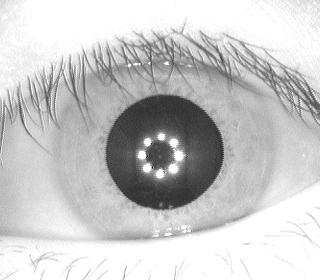
\includegraphics[width=44mm]{tfm-img16}}
\subfigure[S1113R05.jpg]{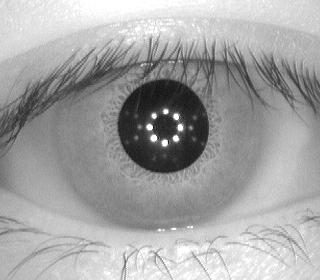
\includegraphics[width=44mm]{tfm-img17}}
\subfigure[S1188L04.jpg]{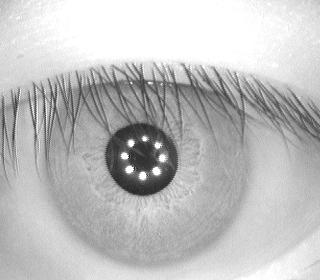
\includegraphics[width=44mm]{tfm-img18}}
\subfigure[S1200R02.jpg]{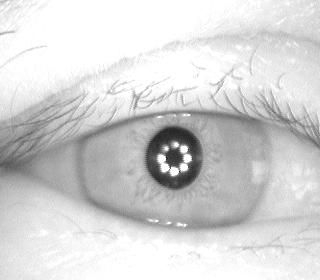
\includegraphics[width=44mm]{tfm-img19}}
\subfigure[S1217L04.jpg]{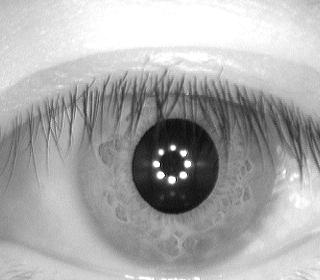
\includegraphics[width=44mm]{tfm-img20}}
\caption{Imágenes de la base de datos CASIA-IrisV4.} \label{fig:señales}
\end{figure}

%----------------------------------------------------------------------------------------

\section{LIP-VIREO}

Es una herramienta multiplataforma empleada en la extracción de características basada en puntos de interés locales sobre la textura de una imagen. Esta desarrollada en C++ y actualmente cuenta con la implementación de ocho detectores de puntos de interés como son \textbf{DoG}, \textbf{LoG}, \textbf{Harris-Laplace}, \textbf{Hessian-Laplace}, \textbf{Harris}, \textbf{Hessian}, \textbf{Fast Hessian} (detector SURF) y \textbf{Dense}. Además cuenta también con un conjunto de descriptores de puntos de interés como \textbf{SIFT}, \textbf{Flip}, \textbf{FIND}, \textbf{PCA-SIFT}, \textbf{SPIN}, \textbf{RIFT}, \textbf{ERIFT}, \textbf{SURF}, \textbf{AoD} y \textbf{LJET}.

Dentro del ámbito de los detectores de puntos de interés, \textbf{Harris} y \textbf{Harris-Laplace} se basan en diferentes funciones para medir la prominencia de la región alrededor de un pixel. Estos detectores están basados principalmente en la matriz de segundo momento para un punto X como se muetra en la siguiente figura.

\begin{figure}[htbp]
\centering
\[
\mu \left ( X,\sigma _{1},  \sigma _{D}\right ) = \sigma ^{2}_{D}g(\sigma _{I}) * \begin{bmatrix}
L^{2}_{x}(X,\sigma _{D}) \:\:\:\: L_{x}L_{y}(X,\sigma _{D}) \\
L_{x}L_{y}(X,\sigma _{D}) \:\:\:\: L^{2}_{y}(X,\sigma _{D})
\end{bmatrix}
\] 
\caption{Matriz de segundo momento para el detector Harris.} 
\end{figure}

donde $\sigma _{I}$ es la escala de integración, $\sigma _{D}$ es la escala de diferenciación y $L_{g}$ es la derivada calculada en la dirección g (x o y). Esta matriz principalmente describe la distribución del gradiente en un vecindario local de un punto X. \\

A diferencia del detector \textbf{Harris}, la matriz de los detectores \textbf{Hessian} y \textbf{Hessian-Laplace} para un punto dado X viene expresada de la siguiente manera. \\

\begin{figure}[htbp]
\centering
\[
H( X,  \sigma) = 
\begin{bmatrix}
L_{xx}(X,\sigma) \:\:\:\: L_{xy}(X,\sigma) \\
L_{xy}(X,\sigma) \:\:\:\: L_{yy}(X,\sigma)
\end{bmatrix}
\]
\caption{Matriz de segundo momento para el detector Hessian (I).} 
\end{figure}

donde $\sigma$  es el parámetro de suavizado Gaussiano. La ecuación siguiente define la prominencia del punto X solamente basado en el determinante de la matriz Hessian. \\

\begin{figure}[htbp]
\centering
\[
H( X, \sigma _{D} ) = 
\begin{bmatrix}
L_{xx}(X,\sigma_{D}) \:\:\:\: L_{xy}(X,\sigma_{D}) \\
L_{xy}(X,\sigma_{D}) \:\:\:\: L_{yy}(X,\sigma_{D})
\end{bmatrix}
\] 
\caption{Matriz de segundo momento para el detector Hessian (II).} 
\end{figure}

\begin{figure}[htbp]
\centering
\[
Hessian(X, \sigma) = det(H(X,\sigma)) x \sigma^4
\]
\caption{Detector Hessian.} 
\end{figure}

El detector \textbf{Laplaciano de Gauss (LoG)} se basa en la siguiente ecuación para medir la prominencia de un punto X. 

\begin{figure}[htbp]
\centering
\[
LoG(X, \sigma_{I}) = \sigma_{I}(L_{xx}(x,\sigma_{I}) + L_{yy}(x,\sigma_{I}))
\]
\caption{Detector LoG.} 
\end{figure}

Los puntos que alcanzan los máximos locales simultáneamente en sus espacio y escala son los que se seleccionan. Comparando a los detectores vistos anteriormente, podemos observar como en este caso la función de prominencia en el espacio X-Y se ha reemplazado con el laplaciano de Gauss, mientras que la función de prominencia en el espacio de escala se mantiene. Es por eso por lo que estos dos detectores pueden compartir puntos de interés similares. \\

La ecuación de la figura anterior (Figura 3.6) realiza una estimación de las segundas derivadas en las direcciones \textit{x} e \textit{y}, lo que implica que el coste de computación sea relativamente alto. Es por eso por lo que se define una manera más eficiente a través de la \textbf{Diferencia de Gauss DoG} ya que esta solamente requiere la convolución de imágenes de manera constante. \\ \\ \\ \\ \\ \\

\begin{figure}[htbp]
\centering
\[
D(x, y, \sigma) = L(x,y,k\sigma) - L(x,y,\sigma)
\]
\caption{Detector DoG.} 
\end{figure} 

donde $\sigma$ es el parámetro de suavizado Gaussiano y \textit{k} es un multiplicador entero. \\ 

\textbf{Fast Hessian} es el detector de características SURF. Su idea básica es calcular la ecuación de la Figura 3.5 de una manera eficiente con la ayuda de imágenes integrales. Para permitir un cálculo rápido, la ecuación de dicha figura ha sido aproximada de la siguiente manera. 

\begin{figure}[htbp]
\centering
\[
Det(H_{approx}) = D_{xx}D_{yy} - (0.9D_{xy})^2
\]
\caption{Detector Fast Hessian.} 
\end{figure}

donde $D_{xx}$, $D_{yy}$ y $D_{xy}$ son todos calculados eficientemente usando cajas de filtros. \\

\textbf{Dense Sampling} es el último de los detectores de puntos de interés que vamos a ver. Este detector ha mostrado un rendimiento considerablemente mejor que los detectores mejor diseñados en tareas de detección de objetos. El ratio por defecto de este detector es de un punto por cada 10 pixeles. \\

Al no ser los puntos de interés suficientemente discriminativos, es necesario disponer de más información para poder comparar dos imágenes. Para realizar esta tarea se utilizan los descriptores, los cuales generan un vector de características sobre un punto a partir del mapa de intensidades de su alrededor. Para ello, el framework \textbf{LIP-VIREO} dispone de un conjunto determinado de métodos y algoritmos capaces de extraer el vector de características correspondiente para cada punto de interés.  \\

El descriptor \textbf{SIFT} y sus respectivas variantes ( \textbf{F-SIFT}, \textbf{PCA-SIFT} y \textbf{FIND} copan la mayoría de los descriptores que proporciona la librería. Además de estos, también se encuentran las implementaciones de descriptores como \textbf{SURF}, \textbf{AoD}, \textbf{SPIN}, \textbf{RIFT}, \textbf{ERIFT} y \textbf{Steerable Filters}. \\

\textbf{SIFT} ha demostrado ser un descriptor efectivo en tareas tales como la clasificación de objetos y la identificación de imágenes ND entre otras. Dado un punto de interés normalizado, SIFT genera un histograma 2-D sobre el área local del punto. Este área local es particionado en bloques como se muestra en la siguiente figura 39. La gradiente de un pixel dentro de cada bloque de partición ha sido cuantificada acorde a su orientación. Antes de cuantificar los contenedores del área local se realiza una rotación sobre la orientación dominante para hacer que la extracción de las características sea invariante a la transformación de rotación. \\

El descriptor \textbf{Flip} es una invariante del mencioando anteriormente \textbf{SIFT}, siendo este capaz de mantener un rendimiento similiar \textbf{SIFT} para casos en los que no está implicado, mientras que lo supera aparentemente en los casos que la operación flip es observada. \\

\textbf{PCA-SIFT} es otra variante de \textbf{SIFT}. En este caso, en vez de cuantificar el campo gradiente, asigna dicho campo a un vector (normalmente de 36 dimensiones) con una matriz PCA entrenada. Antes de realizar el mapeo o asignación, el área local es normalizada para fijarla a un tamaño. El gradiente de cada pixel en el área normalizada es calculado. Esos gradientes son entonces concatenados uno detrás de otro desde la esquina superior izquierda a la esquina inferior derecha. El resultado es un vector de tamaño dos veces el número de píxeles. Este vector es mapeado a una dimensión relativamente baja a través un mapeo con la matriz PCA. \\

El descriptor \textbf{FIND} se propuso como una variante de \textbf{SIFT } que está habilitado con la invariante flip. Al igual que sucede con el descriptor \textbf{SIFT}, también se genera un histograma de gradientes. La mayor diferencia entre ambos descriptores reside en el esquema de partición, ya que este tipo de descriptor permite el solapamiento entre bloques. En esta ocasión, el número de pixeles no es distribuido igualmente en cada bloque como se muestra en la figura 39. Este descriptor llega a ser bastante similar a \textbf{F-SIFT}, excepto que estos confían en diferente información para la normalización y que adoptan diferente esquema de partición. Comparándolo con \textbf{F-SIFT}, tanto el esquema de partición como la orientación estimada que adopta es menos estable, siendo en términos de computación este último más barato. \\

\textbf{Steerable filters} es un descriptor que ha sido usado en muchos contextos. Básicamente son derivadas parciales obtenidas al aplicar series de kernels Gaussianos en el área local. Esta implementación del framework se basa en un kernel centrado alrededor del punto de interés de 41x41. Las derivadas han sido calculadas hasta el cuarto oden. Esto da como resultado un vector de características de dimensión 15 que incluye valores de intensidad de los propios píxeles. \\

El dominio de la intensidad de una imagen \textbf{SPIN} incorporado en este framework es un histograma de dos dimensiones que codifica la distribución de los valores de brillo de la imagen en el vecino mas cercano de un punto particular. El esquema de cuantificación se muestra en la figura siguiente. En este desciptor, las dos dimensiones del histograma son \textit{d}, distancia desde el centro del punto e \textit{i}, el valor de la intensidad. La porción de la imagen spin correspondiente a una determinada distancia \textit{d}, es simplemente el histograma de los valores de intensidad de los píxeles localizados a una distancia \textit{d} desde el centro. Debido a que los parámetros \textbf{d} e \textit{i} son invariantes bajo transformaciones ortogonales de la vecindad de la imagen, las imágenes de giro ofrecen a menudo un apropiada condición de invarianza para representar  áreas normalizadas afínes.\\

En este framework, la imagen \textbf{SPIN} es implementada como un histograma suave, donde cada píxel dentro de la región de soporte contribuye a más de un contenedor. Este tipo de descriptor muestra unos resultados excelentes en el contexto únicamente se producen transformaciones de rotado y volteado. El rendimiento disminuye drásticamente cuando se presentan imágenes con transformación de escala. En este caso, la extracción de característcas del método \textbf{SPIN} podría ser muy lenta (aproximadamente 10 veces más lenta que la implementación \textbf{SIFT}). \\

El descriptor \textbf{SURF} comparte el mismo esquema de partición que \textbf{SIFT}. Sin embargo, en cada bloque, en vez de generar histograma de gradientes, \textbf{SURF} agrega en wavelets Haar de diferentes canales. Los filtros de cajas se emplean para lograr una mayor velocidad. La agregación se realiza en \textit{dx}, |\textit{dx}|, \textit{dy} y |\textit{dy}|. Esto da como resultado un vector de dimensión 64. \\

El propósito de \textbf{AoD} se inspira en el descriptor \textbf{SURF}. La única diferencia que se encuetra entre ambos esta en las cajas de filtros. En \textbf{AoD} estas cajas han sido reemplazadas con derivadas en cada pixel. Debido al mayor coste computacional que supone el cálculo de las derivadas, esto hace que este descriptor sea penalizado y por lo general menos eficiente que el descriptor \textbf{SURF}.  \\

Para obtener una representación complementaria de apariencia local de áreas normalizadas, se presenta un descriptor de rotación invariantes que generaliza al descriptor \textbf{SIFT}. El área local circular normalizada es particionada en anillos concéntricos como se muestra en la última figura. Todos los anillos comparten el mismo ancho. Por esta razón, diferentes anillos cubren diferentes números de píxeles. En otras palabras, los tamaños de los histogramas son diferentes. Aparentemente, los anillos exteriores tiene una mayor cobertura. Para mantener la invarianza de rotación, esta orientación es medida en cada punto relativo a la dirección que apunta hacia afuera desde el centro. Se usan 4 anillos y 8 orientaciones de histograma. Por lo tanto, esto produce descriptores de 32 dimensiones. \\

Este descriptor \textbf{ERIFT} (Enhanced Rotation Invatiant Feature Transform) es una versión mejorada de \textbf{RIFT} (Rotation Invatiant Feature Transform). \textbf{ERIFT} sigue el mismo esquema de partición que \textbf{RIFT} en un área local, pero a diferencia de este, se establece un ancho para cada anillo para asegurar que cada uno de los anillos cubran la misma cantidad de píxeles. Similiar a \textbf{RIFT}, el histograma de orientación del gradiente es calculado dentro de cada anillo. Se usan 8 anillos y 8 histogramas de orientación. La cuantificación es realizada en dos direcciones perpendiculares para cada valor del gradiente. Esto da como resultado finalmente descriptores de dimensión 128. \\

\begin{figure}[htbp]
\centering
\subfigure[SIFT]{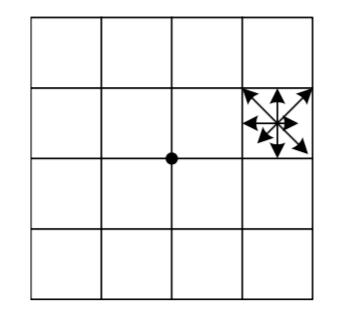
\includegraphics[width=44mm]{tfm-img67}}
\subfigure[GLOH]{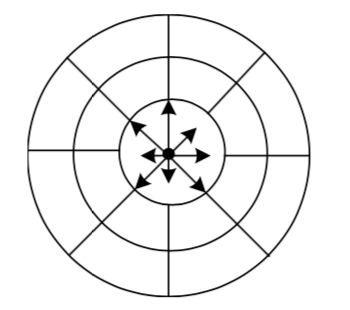
\includegraphics[width=44mm]{tfm-img68}}
\subfigure[RIFT and ERIFT]{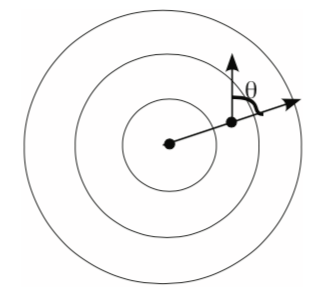
\includegraphics[width=44mm]{tfm-img69}}
\subfigure[SPIN]{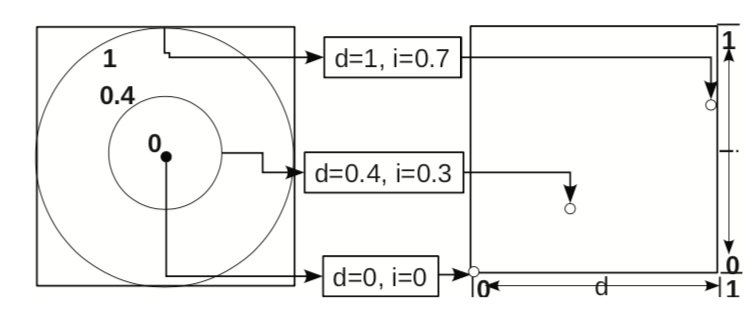
\includegraphics[width=84mm]{tfm-img70}}
\subfigure[FIND]{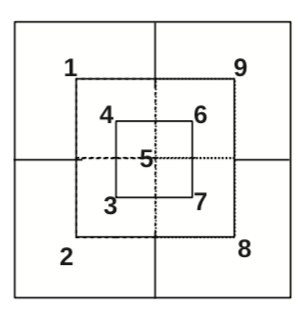
\includegraphics[width=44mm]{tfm-img71}}
\caption{Esquemas de partición para los descriptores SIFT, GLOH, RIFT and ERIFT, SPIN and FIND.} \label{fig:señales}
\end{figure}


%----------------------------------------------------------------------------------------
% Chapter 4

\chapter{Extracción de características del iris en condiciones no ideales} % Main chapter title

\label{Capítulo 4} % For referencing the chapter elsewhere, use \ref{Chapter4} 

%----------------------------------------------------------------------------------------

% Define some commands to keep the formatting separated from the content 
%\newcommand{\keyword}[1]{\textbf{#1}}
%\newcommand{\tabhead}[1]{\textbf{#1}}
%\newcommand{\code}[1]{\texttt{#1}}
%\newcommand{\file}[1]{\texttt{\bfseries#1}}
%\newcommand{\option}[1]{\texttt{\itshape#1}}

%----------------------------------------------------------------------------------------

\section{Introducción}





%----------------------------------------------------------------------------------------

\section{Descripción del método propuesto}



\begin{figure}[htbp]
\centering
\subfigure[S1001L06.jpg]{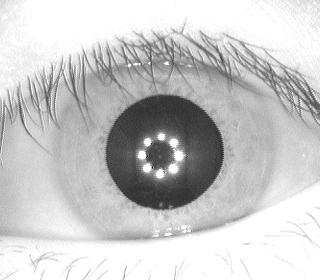
\includegraphics[width=44mm]{tfm-img16}}
\subfigure[S1113R05.jpg]{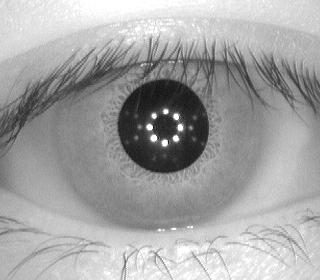
\includegraphics[width=44mm]{tfm-img17}}
\subfigure[S1188L04.jpg]{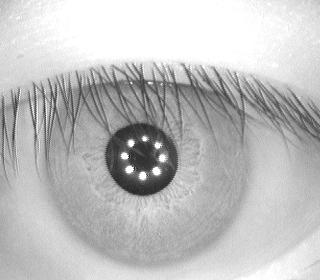
\includegraphics[width=44mm]{tfm-img18}}
\subfigure[S1200R02.jpg]{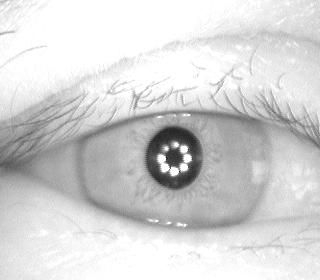
\includegraphics[width=44mm]{tfm-img19}}
\subfigure[S1217L04.jpg]{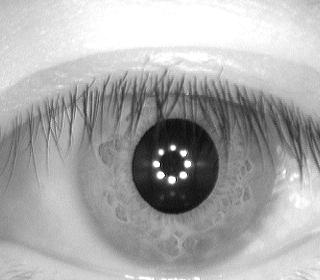
\includegraphics[width=44mm]{tfm-img20}}
\caption{Imágenes de la base de datos CASIA-IrisV4.} \label{fig:señales}
\end{figure}

%---------------------------------------------------------------------------------------- 
% Chapter 5

\chapter{Extracción de características del iris en condiciones no ideales} % Main chapter title

\label{Capítulo 5} % For referencing the chapter elsewhere, use \ref{Chapter5} 

%----------------------------------------------------------------------------------------

% Define some commands to keep the formatting separated from the content 
%\newcommand{\keyword}[1]{\textbf{#1}}
%\newcommand{\tabhead}[1]{\textbf{#1}}
%\newcommand{\code}[1]{\texttt{#1}}
%\newcommand{\file}[1]{\texttt{\bfseries#1}}
%\newcommand{\option}[1]{\texttt{\itshape#1}}

%----------------------------------------------------------------------------------------

\section{Introducción}

De todas las etapas de las que se compone un sistema de reconocimiento de iris la extracción de características se puede destacar como la etapa de mayor importancia siendo una de las áreas mas estudiadas dentro de este campo de investigación, pero que aún a día de hoy presenta cuestiones que requieren de estudios adicionales que ayuden a aumentar el grado de robustez y precisión. Esto hace presentar un nuevo desafío en el reconocimiento del iris en condiciones no ideales, donde las principales tendencias se centran en el estudio relacionado en cuanto a las deformaciones presentadas en la textura y forma del iris. Estas deformaciones son producidas por las degradaciones que sufren las imágenes de iris capturadas en condiciones no ideales que son afectadas por diferentes factores de calidad como iluminación, emborronado, oclusión y perspectiva, entre otros. Este aspecto hace que los sistemas de reconocimiento de iris que son muy dependientes de los detalles de la textura del mismo sean los mas propensos a fallar en las etapas de segmentación y extracción de características, ya que ambas están fuertemente ligadas a dicha textura. Debido a esto, el éxito de acierto en estos sistemas de reconocimiento empeora dando lugar a que se rechacen injustamente a usuarios auténticos por presentar imágenes con mala calidad. \\ \\

Hasta el momento, son dos los tipos de aportaciones realizadas en la extracción de características basadas principalmente en los diferentes tipos de representación de la textura del iris: código binario y vector de valores reales. El trabajo de J. Daugman \cite{Reference15} es la base de los métodos basados en el tipo de representación de código binario. Para la representación del método propuesto en este Trabajo Fin de Master se realizará un proceso de codificación de la información de fase de la transformada 2D Gabor wavelets para obtener el código binario debido a que los datos se presentarán como un vector de valores reales una vez realizada la segmentación. Los métodos basados en representación de la información en forma de vector de valores reales utilizan transformaciones similares, aunque mantienen los valores de los resultados originales en forma de vector de valores reales, es decir, no realizan una transformación binaria de los mismos.\\

Existen 3 principales categorías en las que los métodos de extracción de características pueden ser aplicados: 1) basados en la región del iris completa, 2) basados en regiones de interés y 3) basados en puntos de interés. La primera categoría engloba a los métodos de extracción de categorías tradicionales los cuales extraen características globales y locales de la región completa del iris. La segunda categoría agrupa los métodos que extraen características locales en regiones de interés con la finalidad de superar la falta de información producida principalmente por oclusiones de párpados y pestañas. Son diferentes las regiones en las que se pueden basar estos métodos tales como: la parte superior de la región normalizada del iris, la región delimitada por el collarete del iris, la región anular del iris antes del proceso de normalización de dicha región, etc. La tercerca categoría incluye los métodos de extracción de características basados en puntos de interés que son detectados en el espacio de escala, sobre los que se extraen vectores de valores reales que describen la apariencia alrededor de cada punto de interés. Estos métodos se componen de un detector de puntos de interés y un descriptor que describe la zona alrededor de cada punto de interés. Han sido muy útiles en aplicaciones de reconocimiento de objetos en imágenes afectadas por problemas de oclusión, objetos amontonados, diferentes fuentes de ruido, etc. Aunque este tipo de métodos se comportan bastante bien en el caso de imágenes ruidosas, requiere todavía de mejoras en términos de precisión cuando se producen otro tipo de afectaciones en las imágenes. \\ \\

Aprovechando las ventajas que aportan los métodos de extracción de características basados en puntos de interés, en este Trabajo Fin de Master se propone un nuevo método de extracción de características que se basa en esos tipos de métodos. En definitiva, la finalidad de este Trabajo Fin de Master es la de desarrollar un método de extracción de características basado en puntos de interés para aumentar la robustez y precisión en el reconocimiento de iris en condiciones no ideales frente a otros métodos ya existentes. Este método combina la información obtenida en forma de puntuación desde 3 fuentes de detectores de puntos de interés. Los tres detectores utilizados son: Harris-Laplace \cite{Reference20}, Hessian-Laplace \cite{Reference20} y Fast-Hessian (el detector utilizado por SURF) \cite{Reference21}. Con los puntos de interés localizados por los detectores, se pasa entonces a describir la región alrededor de cada punto de interés a través del descriptor SIFT. De cada una de las fuentes se obtienen las puntuaciones como resultado de comparar imágenes de iris representadas mediante puntos de interés utilizando una distancia propuesta, la cual es una variante restringida de la clásica "proporción de distancias de los vecinos cercanos". Se propone un regla de suma ponderada basada en el ranking de 3 medidas de desempeño (AUC, EER y CRR at Rank-1) para realizar la fusión de las puntuaciones obtenidas mediante las 3 fuentes detectoras de puntos de interés. \\

A través de este nuevo método de extracción de características propuesto se hacen innecesarios los componentes como la segmentación muy precisa del iris o la normalización de la región anular del iris para aumentar el grado de robustez y precisión en el reconocimiento. Este método cuenta con la ventaja de fusionar información de diferentes fuentes, lo cual es una solución eficiente de cara a los problemas prácticos como el ruido en los datos y la no universalidad entre otros. Se desarrollarán experimentaciones exhaustivas en los modos de verficación e identificación sobre la basa de datos CASIA-IrisV4-Interval para demostrar la validez del método propuesto. \\


%----------------------------------------------------------------------------------------

\section{Descripción del método propuesto}

Para la ejecución del método propuesto de extracción de características del iris basado en puntos de interés es necesario que anteriormente se haya segmentado el iris de la imagen. Para realizar este procedimiento se utilizará el método que se definió en el capítulo 4. Una vez segmentado el iris se le aplicará una mejora contraste a la textura del mismo para que de esta forma destaquen los puntos mas interesantes de la imagen de cara al método de extracción de características basado en puntos de interés. \\


\subsection{Tratamiento de la textura del iris}

Antes de aplicar el método de extracción de características propuesto sobre la imagen del iris segmentada se realizará un tratamiento a dichas imagenes con el objetivo de mejorar la textura del iris. La aplicación de este procedimiento se realizará a través de un método de mejora de contraste en imágenes popularmente conocido en este ámbito.  Este método es el llamado ecualización de histograma adaptativo por contraste limitado CLAHE (contrast-limited adaptive histogram equalization) el cual tiene como finalidad la de mejorar el contraste en imágenes de escalas de grises \cite{Reference22}.  El modo de operación de CLAHE es aplicado sobre vecindades de 8x8 llamadas ventanas, cuyo propósito es el de mejorar el contraste en cada ventana de manera que el histrograma de la imagen transformada se puede ajustar a un histrograma plano. Del mismo modo, las ventanas vecinas son combinadas utilizando interpolación bi-linear para elminar los bordes incluidos artificialmente. Es importante ajustar el límite del aumento del contraste, ya que en áreas de píxeles homogéneas puede producir una saturación en la imagen. En la siguiente figura se puede ver el resultado de aplicar dicha transformación a la imagen original.\\ \\ \\

\begin{figure}[htbp]
\centering
\subfigure[S1001L01.jpg]{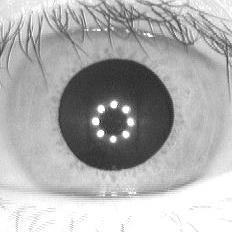
\includegraphics[width=44mm]{tfm-img21}}
\subfigure[S1001L01.jpg]{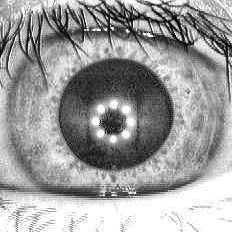
\includegraphics[width=44mm]{tfm-img22}}
\caption{Resultado de la aplicación del método de mejora de constraste CLAHE sobre una imagen de la base de datos CASIA-IrisV4-Internal. (a) Imagen original. (b) Resultado de aplicar el método CLAHE.} \label{fig:señales}
\end{figure}


\subsection{Extracción de las características basada en puntos de interés}

Dentro de los métodos de extracción de características podemos distinguir los que se centran en extraer características locales, normalmente basados en puntos de interés y que presentan un mayor robustez ante problemas de oclusión, objetos superpuestos, diferentes fuentes de ruido y perspectiva, y los métodos que se centran en extraer características globales, los cuales tienen cierta desventaja frente a los anteriores para el reconocimiento de iris en condiciones no ideales. Estos tipos de métodos basados en características globales parten de la desventaja de que no son capaces de diferenciar si un punto o característica pertenece al objeto o al fondo de la escena, requiriendo en estos casos aplicar operaciones adicionales como una segmentación más precisa del iris, lo que resulta bastante complejo en condiciones no ideales. Básicamente, los métodos de extracción de características locales basados en puntos de interés se conforman de un detector de puntos de interés y de un descriptor que describe la región alrededor de cada punto de interés. \\

Los puntos de interés son detectados en el espacio de escala. Para eso nos basamos en el supuesto de que los objetos tienen una propiedad innata en el mundo real por la cual estos sólo existen como entidades con sentido en un cierto rango de escalas. Mediante esta propiedad podemos comprobar como los objetos que son más relevantes en una imagen persisten, y como los menos significativos desaparecen. Para realizar este procedimiento lo que se hace es representar la imagen en múltiples escalas creando para ello un espacio de escala. Este espacio de escala se define como el resultado obtenido de la convolución de una escala variable Gaussiana \textit{G(x, y, z)} con la imagen de entrada \textit{I(x, y)}:\\

\[
L(x,y,\sigma) = G(x,y,\sigma) * I(x,y)
\]

En la siguiente figura se puede ver el efecto de emborronado que produce el cambio brusco de los valores variando el flitro en la función Gaussiana. \\ \\ \\

\begin{figure}[htbp]
\centering
\subfigure[]{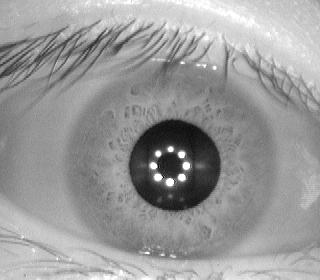
\includegraphics[width=50mm]{tfm-img24}}
\subfigure[]{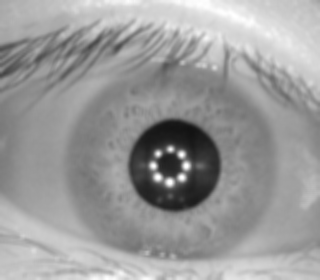
\includegraphics[width=50mm]{tfm-img25}}
\subfigure[]{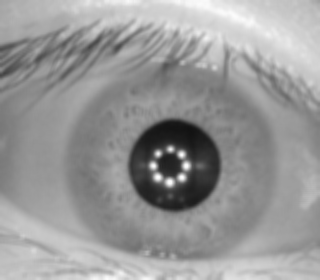
\includegraphics[width=50mm]{tfm-img26}}
\subfigure[]{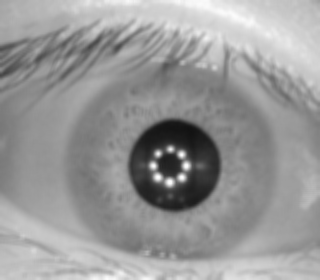
\includegraphics[width=50mm]{tfm-img27}}
\caption{Representación del espacio de escala sobre una imagen de la base de datos CASIA-IrisV4-Internal. (a) Imagen original. (b) $\sigma$ = 3. (c) $\sigma$ = 5. (d) $\sigma$ = 10.} \label{fig:señales}
\end{figure}

Los detectores de puntos de interes se basan en la búsqueda de características tales como esquinas, blobs y regiones dentro de la imagen, identificando en dichos lugares los puntos de interés que no varían en situaciones de transformaciones de escala, perspectiva y/o transformaciones afines. El propósito de los descriptores es el de extraer información discriminante alrededor de los puntos de interés. Estos se clasifican en 3 categorías: basados en distribuciones (SIFT, PCA-SIFT, GLOH, SURF), basados en técnicas de frecuencia espacial (Transformada de Fourier, Transformada de Gabor, Transformada de wavelet) y descriptores diferenciales (Filtros Steerable, Invariante diferencial). \\

El método de extracción de características que se propone en este Trabajo Fin de Master se encuadra dentro de los métodos de extracción de características locales, que como ya se ha visto se componen de un detector de puntos de interés y de un desciptor encargado de describir la región alrededor de cada punto. A diferencia de otros métodos de extracción de características existentes que emplean un único detector de puntos de interés, el método propuesto fusiona 3 detectores dentro del conjunto de los basados en la búsqueda de características en esquinas, blobs y regiones. Para mantener un equilibrio entre los seleccionados de estos tipos de detectores se ha realizado un estudio donde se pueda analizar los resultados que arrojarían utilizando varias combinaciones de estos detectores y descriptores para valorar cual sería la combinación óptima de los mismos \cite{Reference23} \cite{Reference24} \cite{Reference25}. Tras la evaluación investigada sobre las posibles combinaciones de detectores y descriptores, se ha llegado a la conclusión de que el resultado que proporciona un mayor interés en su investigación y que puede ser el más adecuado es el formado por la combinación de los detectores Harris-Laplace (detector de esquina), Hessian-Laplace (detector de blobs) y Fast-Hessian (detector de blobs). De entre todos los descriptores mencionados en el estado del arte, se ha seleccionado el descriptor SIFT como el encargado de caracterizar las regiones alrededor de cada punto de interés detectado debido que es el que mejor se integra con los detectores nombrados anteriormente. Además, este descriptor constituye la base de varios descriptores y como se ve en la siguiente figura representa un mayor grado de precisión frente a los demás descriptores. \\

\begin{figure}[htbp]
\centering
\subfigure{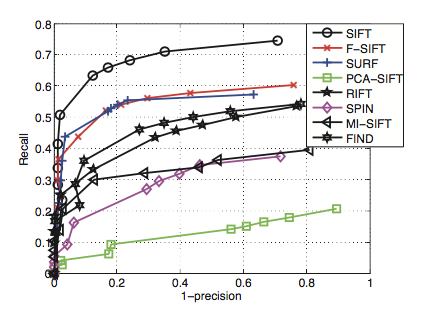
\includegraphics[width=110mm]{tfm-img51}}
\caption{Rendimiento de ocho descriptores diferentes con el detector DoG sobre 8 pares de imágenes que cubren transformaciones como escalado, rotación, cambios en el punto de vista, emborronado, cambios en el ratio de comprensión JPEG y cambios de iluminación.} \label{fig:señales}
\end{figure}


\subsubsection{Harris-Laplace}

El detector Harris \cite{Reference24} se basa principalmente en la matriz de segundo momento que es definida en la siguiente figura para un punto X.

\[
\mu (X, \sigma_{I}, \sigma_{D}) = \sigma_{D}^{2} g(\sigma_{I}) * \begin{bmatrix}
 L_{x}^{2}(X, \sigma_{D}) &  L_{x} L_{y}(X, \sigma_{D}) \\ 
  L_{x} L_{y}(X, \sigma_{D}) & L_{y}^{2}(X, \sigma_{D})
\end{bmatrix}
\]
\captionof{figure}{Ec. 1.1} 

donde $\sigma_{I}$ es la escala de integración, $\sigma_{D}$ es la escala de diferenciación y $ L_{g}$ es la derivada calculada en la dirección g (X o Y). Esta matriz describe principalmente la distribución del gradiente en un vecindario local de un punto X. Las derivadas locales son calculadas con núcleos (kernel) Gaussianos de un tamaño determinado por la escala local $\sigma_{D}$ (escala de diferenciación). Las derivadas son entonces promediadas entre los vecinos cercanos de los puntos por suavizado con una ventana Gaussiana de tamaño $\sigma_{I}$ (escala de integración). Los valores propios de esta matriz presenta dos cambios principales de señal en los vecinos cercanos de un punto. Basado en esta función, el detector Harris favorece a los pixeles que tienen grandes valores de curvatura en ambas direcciones principales. Por lo tanto, la función de selección es definida como muestra la siguiente figura. 

\[
Harris(X, \sigma_{I}, \sigma_{D}) = \left | \mu (X, \sigma_{I}, \sigma_{D}) \right | - \alpha*trace^{2}(\mu (X, \sigma_{I}, \sigma_{D}))
\]
\captionof{figure}{Ec. 1.2} 

donde $\alpha$ es una constante. En consecuencia, un punto de interés local es identificado donde un pixel alcanza un máximo local con respecto a las esquinas. \\

Para lograr la invarianza de escala, una escala apropiada debe ser elegida para cada punto de interés local detectado. Este proceso implica buscar extremos locales en el espacio de escala. En la matriz del segundo momento adaptada a la escala, el parámetro $\sigma_{I}$ determina la escala de la región local centrada en el punto X. Diferentes $\sigma_{I}$ dan como resultado diferentes máximos locales de función. Sin embargo, no todos los máximos locales generados por diferentes $\sigma_{I}$ son válidos.  Para simplificar el problema, $\sigma_{D}$ está relacionado con $\sigma_{I}$ por un ratio constante, por ejemplo, $\sigma_{D}$ = 0.8 · $\sigma_{I}$ . Como resultado, el problema de buscar parámetros apropiados para $\sigma_{D}$ y $\sigma_{I}$, se ha reducido la búsqueda de extremos locales en el espacio de escala. \\

Sin embargo, como indica T.Lindeberg \cite{Reference26}, la ecuación Ec. 1.2 rara vez alcanza los máximos en el espacio de escala. Por el contrario, si se mide la prominencia de la región con la función Laplaciana de Gauss en el espacio de escala, el extremo local en el espacio de escala puede ser definido con mas precisión.

\[
LoG(X, \sigma_{I}) = \sigma_{I}(L_{xx(x, \sigma_{I})} + L_{yy(x, \sigma_{I})})
\]
\captionof{figure}{Ec. 1.3} 

donde $L_{gg}$ indica la derivada de segundo orden en la dirección g. Como resultado, el detector Harris-Laplace en lugar de medir la prominencia para cada pixel como en la ecuación Ec. 1.2 solo, la Ec. 1.3 es también aplicada en cada pixel. Este proceso ha sido repetido en múltiples escalas. Los puntos de interés finales son localizados en el espacio X-Y donde la ecuación Ec. 1.2 alcanza el máximo local y la ecuación Ec. 1.3 alcanza el extremo local simultáneamente. \\


\subsubsection{Hessian-Laplace}

A diferencia del detector Harris, dada la matriz Hessian para un punto X.

\[
H(X, \sigma) = \begin{bmatrix}
 L_{xx}(X, \sigma) &  L_{xy}(X, \sigma)  \\ 
 L_{xy}(X, \sigma)  &  L_{yy}(X, \sigma))
\end{bmatrix}
\]
\captionof{figure}{Ec. 1.4} 

donde $\sigma$ es el parámetro de suavizado Gaussiano. La ecuación Ec. 1.6 define la prominencia de un punto X únicamente basado en el determinante de la matriz de Hessian. 

\[
H(X, \sigma) = \begin{bmatrix}
 L_{xx}(X, \sigma_{D}) &  L_{xy}(X, \sigma_{D})  \\ 
 L_{xy}(X, \sigma_{D})  &  L_{yy}(X, \sigma_{D}))
\end{bmatrix}
\]
\captionof{figure}{Ec. 1.5} 

De manera similiar a Harris-Laplace, se requiere seleccionar un parámetro $\sigma_{d}$ apropiado. Esto implica la construcción de un espacio de escala con la ecuación Ec. 1.5. Los puntos Hessian son por lo tanto definidos en la ecuación Ec. 1.5 que alcanza los extremos locales en el espacio de escala.. \\

Actualmente, para seleccionar apropiadamente $\sigma_{D}$ en el espacio de escala tenemos otra opción nombrada como la función Laplaciana de Gauss. Si los puntos detectados son requeridos para alcanzar el extremo local con la ecuación Ec. 1.3 en el espacio de escala, se define el nuevo detector Hessian-of-Laplacian. 

\[
H(X,\sigma) = det(H(X,\sigma))  *  \sigma^{4}
\]
\captionof{figure}{Ec. 1.6} 

\begin{table}[htbp]
\begin{center}
\end{center}
\end{table}

\begin{table}[htbp]
\begin{center}
\end{center}
\end{table}

\subsubsection{Fast-Hessian}
Fast Hessian es el detector de características SURF \cite{Reference27}. Su idea básica es calcular la ecuación Ec. 1.6 de una manera eficiente con la ayuda de imágenes integrales. Para permitir un cálculo rápido, la ecuación Ec. 1.6 ha sido aproximada a la ecuación Ec. 1.7.

\[
Det(H_{approx}) = D_{xx}D_{yy} - (0.9D_{xy})^{2}
\]
\captionof{figure}{Ec. 1.7} 

donde $D_{xx}$, $D_{yy}$ y $D_{xy}$ todos pueden ser calculados eficientemente usando filtros de caja. La detección es realizada en cuatro escalas y tres octavos (particiones de tamaño 8). Debido a la considerable pérdida en la aproximación, la localización de los puntos de interés en cualquier espacio de escala o espacio X-Y no puede ser precisa. Parecido al detector DoG, la expansión Taylor en la ecuación Ec. 1.7 es adoptada para aproximar la ubicación exacta de los extremos. En la implementación original de SURF, el detector había sido emparejado con el descriptor SURF por la preocupación existente en cuanto a la velocidad. \\


\subsubsection{SIFT}
Se ha demostrado que el descriptor SIFT tiene éxito en varias tareas tales como clasificación de objetos, generación de panorama e identificación de imagen ND. Dada una región normalizada de un punto de interés, SIFT genera un histograma 2-D en la región local. La región local se particiona en bloques. La figura 5.11 muestra el esquema de partición de SIFT. El gradiente de un píxel dentro de cada bloque de partición se ha cuantificado de acuerdo con su orientación. Normalmente, el número de contenedores de cuantificación es 8 \cite{Reference28}. Antes de la cuantificación, la región local es rotada a su orientación dominante. Esta operación permite que las características extraídas sean invariantes a las transformaciones de rotación. La orientación dominante se estima también en función de la cuantización de la orientación en el campo gradiente de la región local. Generalmente, la región usada para calcular la orientación dominante es una pequeña porción de la región local (por ejemplo, una parte concéntrica de la región local con longitud de radio la mitad). Para lograr un mejor rendimiento, el histograma se pondera adicionalmente en primer lugar	 por su longitud de gradiente, y en segundo lugar por una ventana Gaussiana centrada alrededor del punto de interés. \\

\begin{figure}[htbp]
\centering
\subfigure{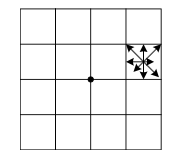
\includegraphics[width=60mm]{tfm-img52}}
\caption{SIFT} \label{fig:señales}
\end{figure}

%---------------------------------------------------------------------------------------- 
% Chapter 6

\chapter{Conclusiones y trabajos futuros} % Main chapter title

\label{Capítulo 6} % For referencing the chapter elsewhere, use \ref{Chapter6} 

%----------------------------------------------------------------------------------------

% Define some commands to keep the formatting separated from the content 
%\newcommand{\keyword}[1]{\textbf{#1}}
%\newcommand{\tabhead}[1]{\textbf{#1}}
%\newcommand{\code}[1]{\texttt{#1}}
%\newcommand{\file}[1]{\texttt{\bfseries#1}}
%\newcommand{\option}[1]{\texttt{\itshape#1}}

%----------------------------------------------------------------------------------------





%----------------------------------------------------------------------------------------

Este trabajo final de Master presentado, propone una nueva alternativa para el reconocimiento de iris en condiciones no ideales. La utilización de esta nueva propuesta aporta varias contribuciones que se traducen principalmente en las siguientes direcciones: aplicar un adecuado tratamiento a las imágenes que resalten más el área del iris para realizar una mejor segmentación, un método basado en análisis de perfiles para la segmentación del iris en base a su centro y sus áreas interna y externa, una aplicación al iris segmentado que ayude a realzar los puntos de interés de dicha región y un nuevo método para la extracción de características del iris basado en un esquema de fusión de 3 fuentes de información. De manera general, todos los objetivos fueron alcanzados y se pudieron comprobar sus resultados. A continuación se presentan con más detalles:

\begin{itemize}
    \item Debido a la diversidad de cada una de las imágenes por el tipo de afectación que padece, se hace muy útil aplicar un tratamiento sobre las mismas que ayude a resaltar el área completa del iris frente al resto de la imagen. Para ello se propuso aplicar un filtro Gaussiano adaptando el umbral del mismo a las condiciones del tipo de imagen en función de su afección. De esta manera se consiguió resaltar los detalles del área del iris y eliminar las afecciones producidas en la imagen por las reflexiones especulares, oclusiones e iluminación variable, lo que consiguió hacer mas robusto el proceso de segmentación del mismo..\\
    
    \item Con el área del iris mas resaltada se pasó a realizar la segmentación de la misma basándose en que el centro del iris se acerca al centro de la propia imagen, por lo que a través de un análisis de perfiles localizamos el centro de dicha área. Con el centro del iris localizado, lo siguiente a realizar era la segmentación de los bordes interno y externo de este. Para dicha operación se utilizó un método que buscaba border circulares sobre un radio mínimo y un radio máximo previamente definidos.\\
    
    \item Se realizón un nuevo tratamiento esta vez a la textura del iris segmentado con el objetivo de mejorarla. El método aplicado en cuestión trata de una mejora de contraste para obtener un histograma ecualizado que ayude a mejorar el contraste de las imágenes de iris. Se hicieron varias pruebas para conseguir ajustar adecuadamente el límite del aumento del contraste y evitar una saturación del mismo. \\
    
    \item Se presentó un nuevo método para la extración de características basado en un esquema de fusión de 3 fuentes de información. Este método es muy apropiado para trabajar con imágenes que tienen una calidad variable producida por las diferentes afectaciones. El esquema de fusión propuesto se basa en las ponderaciones obtenidas  del ranking de medidas de desempeño por las 3 fuentes de informaciones. Los resultados que se obtuvieron indicaron la superioridad del nuevo método propuesto frente al resto de métodos del estado del arte. \\
\end{itemize} 


\section{Trabajos futuros}
Son varias las líneas de investigación aparecidas durante el desarrollo del presente trabajo final de Master entre las que se consideran las siguientes:

\begin{itemize}
	 \item Desarrollar una nueva variante del proceso de segmentación del iris haciéndolo más preciso para que sea capaz de eliminar cualquier tipo de afeccón que no se haya podido eliminar en esta investigación. \\
	 
	 \item Ampliar el tipo de imágenes y sus afecciones para ver el comportamiento del método propuesto frente a diferentes factores de calidad.\\
	 
	  \item Desarrollar una variante para el tratamiento de la textura del iris que ayude a resalta con mayor alcance los puntos de interés del mismo.  \\
	  
	  \item Realizar más pruebas de cómputo en una máquina con características superiores a la empleada en esta investigación que permita reducir los tiempo de cálculo. \\
	  
	  \item Desarrollar una adaptación del método propuesto para que la ejecución del mismo y del resto de algoritmos se realicen en GPU en lugar de CPU cmo hasta ahora para que los tiempo se vean considerablemente reducidos.\\
\end{itemize} 



%----------------------------------------------------------------------------------------
%	THESIS CONTENT - APPENDICES
%----------------------------------------------------------------------------------------

%\appendix % Cue to tell LaTeX that the following "chapters" are Appendices

% Include the appendices of the thesis as separate files from the Appendices folder
% Uncomment the lines as you write the Appendices

%% Appendix A

\chapter{Frequently Asked Questions} % Main appendix title

\label{AppendixA} % For referencing this appendix elsewhere, use \ref{AppendixA}

\section{How do I change the colors of links?}

The color of links can be changed to your liking using:

{\small\verb!\hypersetup{urlcolor=red}!}, or

{\small\verb!\hypersetup{citecolor=green}!}, or

{\small\verb!\hypersetup{allcolor=blue}!}.

\noindent If you want to completely hide the links, you can use:

{\small\verb!\hypersetup{allcolors=.}!}, or even better: 

{\small\verb!\hypersetup{hidelinks}!}.

\noindent If you want to have obvious links in the PDF but not the printed text, use:

{\small\verb!\hypersetup{colorlinks=false}!}.

%\include{Appendices/AppendixB}
%\include{Appendices/AppendixC}

%----------------------------------------------------------------------------------------
%	BIBLIOGRAPHY
%----------------------------------------------------------------------------------------

%\printbibliography[heading=bibintoc]
\bibliography{example.bib}
\bibliographystyle{amsplain}

%----------------------------------------------------------------------------------------

\end{document}  
